\documentclass[12pt,twoside]{report}

\newcommand{\reporttitle}{Generating Interactive WebSocket Applications in TypeScript}
\newcommand{\reportauthor}{Anson Miu}
\newcommand{\reporttype}{MEng Individual Project}
\newcommand{\supervisor}{Prof. Nobuko Yoshida}
\newcommand{\sndmarker}{Dr. Iain Phillips}
\newcommand{\cid}{your college-id number}

% include files that load packages and define macros
%%%%%%%%%%%%%%%%%%%%%%%%%%%%%%%%%%%%%%%%%
% University Assignment Title Page 
% LaTeX Template
% Version 1.0 (27/12/12)
%
% This template has been downloaded from:
% http://www.LaTeXTemplates.com
%
% Original author:
% WikiBooks (http://en.wikibooks.org/wiki/LaTeX/Title_Creation)
%
% License:
% CC BY-NC-SA 3.0 (http://creativecommons.org/licenses/by-nc-sa/3.0/)
% 
% Instructions for using this template:
% This title page is capable of being compiled as is. This is not useful for 
% including it in another document. To do this, you have two options: 
%
% 1) Copy/paste everything between \begin{document} and \end{document} 
% starting at \begin{titlepage} and paste this into another LaTeX file where you 
% want your title page.
% OR
% 2) Remove everything outside the \begin{titlepage} and \end{titlepage} and 
% move this file to the same directory as the LaTeX file you wish to add it to. 
% Then add \input{./title_page_1.tex} to your LaTeX file where you want your
% title page.
%
%----------------------------------------------------------------------------------------
%	PACKAGES AND OTHER DOCUMENT CONFIGURATIONS
%----------------------------------------------------------------------------------------
\usepackage{ifxetex}
\usepackage{textpos}
\usepackage[sort,comma]{natbib}
\usepackage{kpfonts}
\usepackage[a4paper,hmargin=2.8cm,vmargin=2.0cm,includeheadfoot]{geometry}
\usepackage{ifxetex}
\usepackage{stackengine}
\usepackage{tabularx,longtable,multirow,subfigure,caption}%hangcaption
\usepackage{fncylab} %formatting of labels
\usepackage{fancyhdr}
\usepackage{color}
\usepackage[tight,ugly]{units}
\usepackage{url}
\usepackage{float}
\usepackage[english]{babel}
\usepackage{amsmath}
\usepackage{graphicx}
\usepackage[colorinlistoftodos]{todonotes}
\usepackage{dsfont}
\usepackage{epstopdf} % automatically replace .eps with .pdf in graphics
\usepackage{backref}
\usepackage{array}
\usepackage{latexsym}
\usepackage{etoolbox}

\usepackage{enumerate} % for numbering with [a)] format 

\usepackage{multicol}
\usepackage{setspace}



\ifxetex
\usepackage{fontspec}
\setmainfont[Scale=.8]{OpenDyslexic-Regular}
\else
\usepackage[pdftex,pagebackref,hypertexnames=false,colorlinks]{hyperref} % provide links in pdf
\hypersetup{pdftitle={},
  pdfsubject={}, 
  pdfauthor={\reportauthor},
  pdfkeywords={}, 
  pdfstartview=FitH,
  pdfpagemode={UseOutlines},% None, FullScreen, UseOutlines
  bookmarksnumbered=true, bookmarksopen=true, colorlinks,
    citecolor=black,%
    filecolor=black,%
    linkcolor=black,%
    urlcolor=black}
\usepackage[all]{hypcap}
\fi

\usepackage{tcolorbox}

% various theorems
\usepackage{amsthm}
\theoremstyle{plain}
\newtheorem{lemma}{Lemma}
\newtheorem{theorem}{Theorem}

\theoremstyle{definition}
\newtheorem{definition}{Definition}

\newtheoremstyle{proof}% name
  {\topsep}% space above
  {\topsep}% space below
  {}% body font
  {}% indent amount
  {\itshape}% theorem head font
  {.}% punctuation after theorem head
  {.5em}% space after theorem head
  {\thmname{#1}\thmnumber{ #2}\thmnote{ (#3)}}% theorem head spec
\theoremstyle{proof}
\newtheorem*{remark}{Remark}
\newtheorem*{thmproof}{Proof}

% example-environment
\newenvironment{example}[1][]
{ 
\vspace{4mm}
\noindent\makebox[\linewidth]{\rule{\hsize}{1.5pt}}
\textbf{Example #1}\\
}
{ 
\noindent\newline\makebox[\linewidth]{\rule{\hsize}{1.0pt}}
}



%\renewcommand{\rmdefault}{pplx} % Palatino
% \renewcommand{\rmdefault}{put} % Utopia

\ifxetex
\else
\renewcommand*{\rmdefault}{bch} % Charter
\renewcommand*{\ttdefault}{cmtt} % Computer Modern Typewriter
%\renewcommand*{\rmdefault}{phv} % Helvetica
%\renewcommand*{\rmdefault}{iwona} % Avant Garde
\fi

\setlength{\parindent}{1em}  % indentation of paragraph


\setlength{\headheight}{14.5pt}
\pagestyle{fancy}
\fancyfoot[ER,OL]{\thepage}%Page no. in the left on
                                %odd pages and on right on even pages
\fancyfoot[OC,EC]{\sffamily }
\renewcommand{\headrulewidth}{0.1pt}
\renewcommand{\footrulewidth}{0.1pt}
\captionsetup{margin=10pt,font=small,labelfont=bf}


%--- chapter heading

\def\@makechapterhead#1{%
  \vspace*{10\p@}%
  {\parindent \z@ \raggedright %\sffamily
        %{\Large \MakeUppercase{\@chapapp} \space \thechapter}
        %\\
        %\hrulefill
        %\par\nobreak
        %\vskip 10\p@
    \interlinepenalty\@M
    \Huge \bfseries 
    \thechapter \space\space #1\par\nobreak
    \vskip 30\p@
  }}

%---chapter heading for \chapter*  
\def\@makeschapterhead#1{%
  \vspace*{10\p@}%
  {\parindent \z@ \raggedright
    \sffamily
    \interlinepenalty\@M
    \Huge \bfseries  
    #1\par\nobreak
    \vskip 30\p@
  }}
  



% %%%%%%%%%%%%% boxit
\def\Beginboxit
   {\par
    \vbox\bgroup
	   \hrule
	   \hbox\bgroup
		  \vrule \kern1.2pt %
		  \vbox\bgroup\kern1.2pt
   }

\def\Endboxit{%
			      \kern1.2pt
		       \egroup
		  \kern1.2pt\vrule
		\egroup
	   \hrule
	 \egroup
   }	

\newenvironment{boxit}{\Beginboxit}{\Endboxit}
\newenvironment{boxit*}{\Beginboxit\hbox to\hsize{}}{\Endboxit}



\allowdisplaybreaks

\makeatletter
\newcounter{elimination@steps}
\newcolumntype{R}[1]{>{\raggedleft\arraybackslash$}p{#1}<{$}}
\def\elimination@num@rights{}
\def\elimination@num@variables{}
\def\elimination@col@width{}
\newenvironment{elimination}[4][0]
{
    \setcounter{elimination@steps}{0}
    \def\elimination@num@rights{#1}
    \def\elimination@num@variables{#2}
    \def\elimination@col@width{#3}
    \renewcommand{\arraystretch}{#4}
    \start@align\@ne\st@rredtrue\m@ne
}
{
    \endalign
    \ignorespacesafterend
}
\newcommand{\eliminationstep}[2]
{
    \ifnum\value{elimination@steps}>0\leadsto\quad\fi
    \left[
        \ifnum\elimination@num@rights>0
            \begin{array}
            {@{}*{\elimination@num@variables}{R{\elimination@col@width}}
            |@{}*{\elimination@num@rights}{R{\elimination@col@width}}}
        \else
            \begin{array}
            {@{}*{\elimination@num@variables}{R{\elimination@col@width}}}
        \fi
            #1
        \end{array}
    \right]
    & 
    \begin{array}{l}
        #2
    \end{array}
    &%                                    moved second & here
    \addtocounter{elimination@steps}{1}
}
\makeatother

%% Fast macro for column vectors
\makeatletter  
\def\colvec#1{\expandafter\colvec@i#1,,,,,,,,,\@nil}
\def\colvec@i#1,#2,#3,#4,#5,#6,#7,#8,#9\@nil{% 
  \ifx$#2$ \begin{bmatrix}#1\end{bmatrix} \else
    \ifx$#3$ \begin{bmatrix}#1\\#2\end{bmatrix} \else
      \ifx$#4$ \begin{bmatrix}#1\\#2\\#3\end{bmatrix}\else
        \ifx$#5$ \begin{bmatrix}#1\\#2\\#3\\#4\end{bmatrix}\else
          \ifx$#6$ \begin{bmatrix}#1\\#2\\#3\\#4\\#5\end{bmatrix}\else
            \ifx$#7$ \begin{bmatrix}#1\\#2\\#3\\#4\\#5\\#6\end{bmatrix}\else
              \ifx$#8$ \begin{bmatrix}#1\\#2\\#3\\#4\\#5\\#6\\#7\end{bmatrix}\else
                 \PackageError{Column Vector}{The vector you tried to write is too big, use bmatrix instead}{Try using the bmatrix environment}
              \fi
            \fi
          \fi
        \fi
      \fi
    \fi
  \fi 
}  
\makeatother

\robustify{\colvec}

%%% Local Variables: 
%%% mode: latex
%%% TeX-master: "notes"
%%% End: 
 % various packages needed for maths etc.
% quick way of adding a figure
\newcommand{\fig}[3]{
 \begin{center}
 \scalebox{#3}{\includegraphics[#2]{#1}}
 \end{center}
}

%\newcommand*{\point}[1]{\vec{\mkern0mu#1}}
\newcommand{\ci}[0]{\perp\!\!\!\!\!\perp} % conditional independence
\newcommand{\point}[1]{{#1}} % points 
% \renewcommand{\vec}[1]{{\boldsymbol{{#1}}}} % vector
\newcommand{\mat}[1]{{\boldsymbol{{#1}}}} % matrix
\newcommand{\R}[0]{\mathds{R}} % real numbers
\newcommand{\Z}[0]{\mathds{Z}} % integers
\newcommand{\N}[0]{\mathds{N}} % natural numbers
\newcommand{\nat}[0]{\mathds{N}} % natural numbers
\newcommand{\Q}[0]{\mathds{Q}} % rational numbers
\ifxetex
\newcommand{\C}[0]{\mathds{C}} % complex numbers
\else
\newcommand{\C}[0]{\mathds{C}} % complex numbers
\fi
\newcommand{\tr}[0]{\text{tr}} % trace
\renewcommand{\d}[0]{\mathrm{d}} % total derivative
\newcommand{\inv}{^{-1}} % inverse
\newcommand{\id}{\mathrm{id}} % identity mapping
\renewcommand{\dim}{\mathrm{dim}} % dimension
\newcommand{\rank}[0]{\mathrm{rk}} % rank
\newcommand{\determ}[1]{\mathrm{det}(#1)} % determinant
\newcommand{\scp}[2]{\langle #1 , #2 \rangle}
\newcommand{\kernel}[0]{\mathrm{ker}} % kernel/nullspace
\newcommand{\img}[0]{\mathrm{Im}} % image
\newcommand{\idx}[1]{{(#1)}}
\DeclareMathOperator*{\diag}{diag}
\newcommand{\E}{\mathds{E}} % expectation
\newcommand{\var}{\mathds{V}} % variance
\newcommand{\gauss}[2]{\mathcal{N}\big(#1,\,#2\big)} % gaussian distribution N(.,.)
\newcommand{\gaussx}[3]{\mathcal{N}\big(#1\,|\,#2,\,#3\big)} % gaussian distribution N(.|.,.)
\newcommand{\gaussBig}[2]{\mathcal{N}\left(#1,\,#2\right)} % see above, but with brackets that adjust to the height of the arguments
\newcommand{\gaussxBig}[3]{\mathcal{N}\left(#1\,|\,#2,\,#3\right)} % see above, but with brackets that adjust to the height of the arguments
\DeclareMathOperator{\cov}{Cov} % covariance (matrix) 
\ifxetex
\renewcommand{\T}[0]{^\top} % transpose
\else
\newcommand{\T}[0]{^\top}
\fi
% matrix determinant
\newcommand{\matdet}[1]{
\left|
\begin{matrix}
#1
\end{matrix}
\right|
}



%%% various color definitions
\definecolor{darkgreen}{rgb}{0,0.6,0}

\newcommand{\blue}[1]{{\color{blue}#1}}
\newcommand{\red}[1]{{\color{red}#1}}
\newcommand{\green}[1]{{\color{darkgreen}#1}}
\newcommand{\orange}[1]{{\color{orange}#1}}
\newcommand{\magenta}[1]{{\color{magenta}#1}}
\newcommand{\cyan}[1]{{\color{cyan}#1}}


% redefine emph
\renewcommand{\emph}[1]{\blue{\bf{#1}}}

% place a colored box around a character
\gdef\colchar#1#2{%
  \tikz[baseline]{%
  \node[anchor=base,inner sep=2pt,outer sep=0pt,fill = #2!20] {#1};
    }%
}%

%%%%%%%%%%%%%%%%%%%%%%%%%%%%%%%

\usepackage{ bm }					% \bm
\usepackage{ cmll }				% \with
\usepackage{ mathtools }		% \mathmakebox

% GENERAL
\newcommand{\role}[1]{
{\color{blue}\bm{\mathsf{#1}}}
}
\newcommand{\mrole}[1]{
{\mathtt{#1}}
}
\newcommand{\mroles}[2]{
{\mrole{#1}\mrole{#2}}
}
\newcommand{\pt}[1]{
{\textnormal{\texttt{pt}}\left({#1}\right)}
}
\newcommand{\rulename}[1]{
[\textsc{#1}]
}
\newcommand{\hlrulename}[1]{
\hl{[\textsc{#1}]}
}
\newcommand{\projconf}[1]{
{\left\langle{#1}\right\rangle}
}
\newcommand{\subtype}{
\prec
}

% NEW GENERAL
\newcommand{\centroidop}{\circledast}
\newcommand{\centroid}[2]{
{#1} \centroidop \mrole{#2}
}

% GLOBAL TYPES
\newcommand{\tend}{\textnormal{\texttt{end}}}
\newcommand{\trecvar}{\textnormal{\texttt{t}}}
\newcommand{\trec}[1]{\mu\trecvar.{#1}}
\newcommand{\gcommone}[3]{
\mrole{#1} \to \mrole{#2}. ~ {#3} :
}
\newcommand{\gcomm}[4]{
\mrole{#1} \to \mrole{#2} : \left\{ {#3} \right\}_{#4}
}
\newcommand{\gtrans}[5]{
\mrole{#1} \rightsquigarrow \mrole{#2}. ~ {#3} : \left\{ {#4} \right\}_{#5}
}
\newcommand{\wf}[1]{
\textnormal{\texttt{wellFormed}}\left(#1\right)
}
\newcommand{\proj}[2]{
{#1} \projop \mrole{#2}
}
\newcommand{\projop}{\upharpoonright}
\newcommand{\mergeop}{
\sqcap
}
\newcommand{\MERGEOP}{
{\mbox{\LARGE$\sqcap$}}
}
\newcommand{\tmerge}[2]{
{#1}\,{\mergeop}\,{#2}
}

% NEW GLOBAL TYPES
\newcommand{\grouteone}[4]{
\mrole{#1} \xrightarrow[\mrole{#3}]{} \mrole{#2}. ~ {#4} :
}
\newcommand{\groute}[5]{
\mrole{#1} \xrightarrow[\mrole{#3}]{} \mrole{#2} : \left\{ {#4} \right\}_{#5}
}
\newcommand{\gtransroute}[6]{
\mrole{#1} \underset{\mrole{#3}}{\rightsquigarrow} \mrole{#2}. ~ {#4} : \left\{ {#5} \right\}_{#6}
}
\newcommand{\wfnew}[2]{
\textnormal{\texttt{wellFormed}}\left(#1, \mrole{#2}\right)
}

% LOCAL TYPES
\newcommand{\tbra}[3]{
\mrole{#1} \with \left\{ #2 \right\}_{#3}
}
\newcommand{\tsel}[3]{
\mrole{#1} \oplus \left\{ {#2} \right\}_{#3}
}
\newcommand{\tselone}[2]{
\mrole{#1} \oplus {#2}
}
\newcommand{\lty}[1]{
T_{\mrole{#1}}
}
\newcommand{\pinP}{
{\mrole{p} \in \mathcal{P}}
}
\newcommand{\qqinP}{
{\mroles{q}{q'} \in \mathcal{P}}
}

% NEW LOCAL TYPES
\newcommand{\router}[4]{
\left(\mrole{#1} \hookrightarrow \mrole{#2}: \left\{{#3}\right\}_{#4}\right)
}
\newcommand{\routerone}[4]{
\texttt{route}\left(\mrole{#1} \hookrightarrow \mrole{#2}: {#3}.~{#4}\right)
}
\newcommand{\routertrans}[5]{
\left(\mrole{#1} \looparrowright \mrole{#2}. ~ {#3} : \left\{{#4}\right\}_{#5}\right)
}

\newcommand{\tselproxy}[4]{
\tsel{\mrole{#1}_{\mrole{#2}}}{#3}{#4}
}

\newcommand{\tbraproxy}[4]{
\tbra{\mrole{#1}_{\mrole{#2}}}{#3}{#4}
}

% LTS
\newcommand{\aout}[3]{
\mrole{#1}\mrole{#2}!{#3}
}
\newcommand{\ain}[3]{
\mrole{#1}\mrole{#2}?{#3}
}
\newcommand{\subj}[1]{
\text{subj}({#1})
}
\newcommand{\treduce}[3]{
{#1} \xrightarrow{\mathmakebox[1em]{#3}} {#2} 
}
\newcommand{\treducelong}[3]{
{#1} \xrightarrow{\mathmakebox[3.5em]{#3}} {#2} 
}

% NEW LTS
\newcommand{\via}[2]{
{\texttt{via}_{\mrole{#1}}({#2})}
} % short-hand notation and macros


\usepackage[nottoc]{tocbibind}
\setcitestyle{numbers}
	
% Change table/figure counter
\usepackage{chngcntr}

% Highlighting
\usepackage{soul}

% Graphics path
\graphicspath{ {figures/} }

\usepackage{underscore}

\usepackage{listings}

% Fancy names
\newcommand{\fancyname}[1]{\textsc{#1}}
\newcommand{\trole}[1]{\texttt{#1}}
\newcommand{\tmsg}[1]{\texttt{#1}}
\newcommand{\tprotocol}[1]{\textsc{#1}}

% Nicer references
\usepackage[noabbrev, capitalise]{cleveref}

% Font?
%\usepackage{ascii}
%\usepackage[T1]{fontenc}
%\renewcommand\ttfamily{\asciifamily}


% Includes

% Proof trees
%\usepackage{amsthm}
%\theoremstyle{plain}
%
%\newtheorem{thm}{Theorem}[section]
%\newtheorem{cor}{Corollary}[theorem]
%\newtheorem{lem}[theorem]{Lemma}
%\usepackage{proof}
\usepackage{bussproofs}

% Code listing

\lstdefinelanguage{Scribble}{
  keywords={module, type, from, as, global,protocol, role, to, choice, at, or, do},
  keywordstyle=\color{blue}\bfseries,
  identifierstyle=\color{black},
  sensitive=false,
  comment=[l]{//},
  morecomment=[s]{/*}{*/},
  commentstyle=\color{darkgray}\ttfamily,
  stringstyle=\color{purple}\ttfamily,
  morestring=[b]',
  morestring=[b]"
}
\lstdefinelanguage{JavaScript}{
  keywords={typeof, new, true, false, catch, function, return, null, catch, switch, var, if, in, while, do, else, case, break, class, export, boolean, throw, implements, import, this, const, let, extends, async, await, namespace, type, abstract, any, number, string, instanceof, typeof, declare, never,enum,constructor,public,private,void,super,undefined},
  keywordstyle=\color{blue}\bfseries,
%  ndkeywords={class, export, boolean, throw, implements, import, this},
%  ndkeywordstyle=\color{darkgray}\bfseries,
  identifierstyle=\color{black},
  sensitive=true,
  comment=[l]{//},
  morecomment=[s]{/*}{*/},
  commentstyle=\color{darkgray}\ttfamily,
  stringstyle=\color{purple}\ttfamily,
  morestring=[b]',
  morestring=[b]"
}
\lstdefinelanguage{Python}{
  keywords={class, self, def, cls, int, str, bool, pass, return, from, import, and, if, else, None, is, not},
  keywordstyle=\color{blue}\bfseries,
  identifierstyle=\color{black},
  comment=[l]{\#},
  commentstyle=\color{darkgray}\ttfamily,
  stringstyle=\color{purple}\ttfamily,
  morestring=[b]',
  morestring=[b]"
}
\lstset{
	basicstyle=\footnotesize\ttfamily,
	numberstyle=\tiny\ttfamily,
	numbers=left,
	frame=single,
	tabsize=4,
    xleftmargin=1.25em,
    framexrightmargin=-0.25em,
    escapeinside={(*@}{@*)}
}
\def\lstonelinejs{\lstinline[language=javascript,basicstyle=\ttfamily]}

% Figure and table counter
\usepackage{chngcntr}
\counterwithout{figure}{chapter}
\counterwithout{table}{chapter}

% Commands
%\newcommand{\term}[1]{\textit{#1}}
%\newcommand{\mathref}[1]{\textsection #1}
%
%\newcommand{\rulename}[1]{[\textsc{#1}]}
%
%\newcommand{\piin}[2]{#1(#2)}
%\newcommand{\piout}[2]{\bar{#1}\langle #2 \rangle }
%\newcommand{\parti}[1]{{\color{blue}\mathbf{#1}}}
%
%\newcommand{\send}[2]{#1!\langle #2 \rangle}
%\newcommand{\recv}[2]{#1?(#2)}
%\newcommand{\bra}[2]{#1 \rhd \left\{#2\right\}}
%\newcommand{\sel}[3]{#1 \lhd #2 \langle #3 \rangle}
%
%\newcommand{\tysend}[2]{#1![#2]}
%\newcommand{\tyrecv}[2]{#1?[#2]}
%\newcommand{\tybra}[2]{#1 \& \left\{#2\right\}}
%\newcommand{\tysel}[2]{#1 \oplus \left\{#2\right\}}


% Typewriter font
% \renewcommand{\ttdefault}{pcr} % selects Courier font

% Citation style
\setcitestyle{square}


%%%%%%%%%%%%%%%%%%%%%%%%%%%%

\begin{document}
% front page
% Last modification: 2016-09-29 (Marc Deisenroth)
\begin{titlepage}

\newcommand{\HRule}{\rule{\linewidth}{0.5mm}} % Defines a new command for the horizontal lines, change thickness here


%----------------------------------------------------------------------------------------
%	LOGO SECTION
%----------------------------------------------------------------------------------------


\includegraphics[width = 4cm]{./figures/imperial}\\[0.5cm] 

\begin{center} % Center remainder of the page

%----------------------------------------------------------------------------------------
%	HEADING SECTIONS
%----------------------------------------------------------------------------------------
\textsc{\LARGE \reporttype}\\[1.5cm] 
\textsc{\Large Imperial College London}\\[0.5cm] 
\textsc{\large Department of Computing}\\[0.5cm] 
%----------------------------------------------------------------------------------------
%	TITLE SECTION
%----------------------------------------------------------------------------------------

\HRule \\[0.4cm]
{ \huge \bfseries \reporttitle}\\ % Title of your document
\HRule \\[1.5cm]
\end{center}
%----------------------------------------------------------------------------------------
%	AUTHOR SECTION
%----------------------------------------------------------------------------------------

\noindent
\begin{minipage}{.5\linewidth}
\begin{flushleft} \large
\textit{Author:}\\
\reportauthor
\end{flushleft}
\end{minipage}%
\begin{minipage}{.5\linewidth}
\begin{flushright} \large
\textit{Supervisor:}\\
\supervisor
\end{flushright}
\begin{flushright} \large
\textit{Second Marker:}\\
\sndmarker
\end{flushright}
\end{minipage}

\vspace{2cm}
\makeatletter
\centering
\@date 


\vfill % Fill the rest of the page with whitespace



\makeatother


\end{titlepage}



%%%%%%%%%%%%%%%%%%%%%%%%%%%% 

\begin{abstract}
This is an abstract.
\end{abstract}

\renewcommand{\abstractname}{Acknowledgements}

\begin{abstract}

I would like to thank Prof. Nobuko Yoshida,
Fangyi Zhou and Dr. Francisco Ferreira for their
continuous support, encouragement and motivation
during the project. 
I extend my gratitude to the members
of the Mobility Reading Group.
Their regular meetings have been a source
of inspiration for me, and helped me spark new ideas
to incorporate into the project.
I would also like to thank Prof. Peter Pietzuch
for supporting me as my personal tutor
throughout the degree.
\\

I would like to thank all the friends I have made
throughout my time at Imperial.
In particular, to the friends under the namespace
labelled \textit{Reply 404} at the time of writing:
I am forever grateful for every bit of shared memory
over the past four years.
\\

Finally, I would like to thank my family
for their unconditional love and support throughout my life,
and encouraging me to pursue a degree abroad.

\end{abstract}

%%%%%%%%%%%%%%%%%%%%%%%%%%%% 

\tableofcontents

%%%%%%%%%%%%%%%%%%%%%%%%%%%% Main document

\chapter{Introduction}

\section{Motivation}

\paragraph{Note: from PLACES}

% Rise of distributed programs -> main challenges
% How to ensure correctness in general: type system, data types
% Type discipline for concurrent programs - behavioural types (--> session types)
% Mainstream example of distirbuted programs: web services (microservice architecture), interactive web application; 
% Objective: 

Modern interactive web applications aim to 
provide a highly responsive user experience by 
minimising the communication latency between clients and servers. 
Whilst the \textit{HTTP} request-response model is 
sufficient for retrieving static assets, applying the same 
stateless communication approach for interactive use cases 
(such as multiplayer games) introduces undesirable 
performance overhead from having to frequently set up 
new connections for client-server interactions. 
Developers have since adopted other communication 
transport abstractions over HTTP connections such as the WebSockets protocol \cite{WebSocketRFC} to enjoy low-latency full-duplex 
client-server communication in their applications over 
a single persistent connection. 
Enabling more complex communication patterns caters for 
more interactive use cases, but introduces additional 
concerns to the developer with respect to implementation correctness.

% Example: noughts and crosses
Consider a classic turn-based board game of \textit{Noughts and Crosses} 
between two players. Both players are identified by either noughts or crosses 
respectively, and take turns to place a mark on an unoccupied cell 
of a 3-by-3 grid until one player wins (when their markers form 
one straight line on the board) or a stalemate is reached 
(when all cells are occupied). A web-based implementation may 
involve players connected to a game server via WebSocket connections 
and interacting with the game from their web browser, which serve 
a \textit{single-page application} (SPA) of the game client written 
in a popular framework like \textit{React.js} \cite{React}. 
SPAs feature a single HTML page and dynamically renders content 
via JavaScript in the browser. 
Players take turns to make a move on the game board and the server 
implements the game logic to progress the game forward until 
a result (either a win/loss or draw) can be declared. 

Whilst WebSockets make this web-based implementation possible, 
it introduces the developer to a new family of communication errors
(in addition to the usual testing for game logic correctness), 
even for this simple game:
we highlight just a few:

\begin{itemize}

\item
\textbf{Deadlocks:} how can we prevent both players waiting for 
each other to make a move at the same time?

\item 
\textbf{Communication mismatches:} what if player 1 sends
a boolean to the game server instead of board coordinates?

\item
\textbf{Channel linearity:} if the game server takes time
to update the game logic and respond to the players, what if 
player 1 clicks the same cell twice and sends the coordinates twice?

\end{itemize}

The complexity of these errors, which correlate to the complexity of tests 
required against these errors, scale with the complexity of the 
communication patterns involved. Over-reliance on integration testing
to attempt to expose communication-related bugs will also slow the
development process, not to mention that the time taken for these
integration tests would scale with the number of roles involved.
A localised, static way for verifying communication correctness would
be highly desirable.

\textit{Multiparty Session Types} (MPST) \cite{MPST} provide 
a framework for formally specifying a structured communication pattern 
between concurrent processes and verifying implementations for 
correctness with respect to the communications aspect. 
By specifying the client-server interactions of our game as a protocol 
and verifying the implementations against the protocol for well-formedness, 
MPST theory guarantees well-formed implementations to be 
free from communication errors.

Existing work \cite{MVU2020,PureScript2019} that 
adapt the MPST framework for web development
acknowledge the limitations of JavaScript -- the language of the browser --
in providing static type-level guarantees, and proceed to use
languages equipped with stronger type systems that compile to JavaScript.
This comes at the cost of a learning curve for the developer,
and limits its utility in the mainstream web development space.

Among the many languages that compile to JavaScript,
TypeScript stands out as the most intuitive to use as it is defined
to be a \textit{superset} of JavaScript. It provides developers
with type-safety through its gradual, structural type system.
Whilst some \cite{MVU2020} point out this limits its usability for
encoding multiparty session types, we believe that the language
offers sufficient features that we can use to provide developers with
communication safety guarantees whilst preserving a flexible, natural
and idiomatic workflow. By building our work upon TypeScript, we
work towards incorporating MPST into mainstream web development,
which reduces development time by programmatically verifying 
implementations for communication correctness.

\section{Objectives}

\section{Contributions}

In this project, we develop and present an
MPST-based framework for developing full-stack
interactive TypeScript applications over WebSocket transport.

We motivate our API generation approach from 
\cite{Hybrid2016,PureScript2019} to generate TypeScript APIs
from a Scribble protocol specification.
Developers write their full-stack applications
by implementing the generated APIs, and can enjoy 
communication safety guarantees by construction.
We explain how our session type encodings target the Node.js
server-side runtime and React.js framework in
\cref{chap:node,chap:react} for server-side
and browser-side endpoints respectively.

In particular, we present a novel approach for integrating
session types into web-based GUI programming based on
translating the theory on model types \cite{MVU2020}
to idiomatic practices on the React.js framework.
With respect to session type theory, implementations using
the generated APIs statically enjoy linear channel usage
guarantees and affine channel usage guarantees for back-end
and front-end targets respectively.

Compared to previous work, we are not only able to
\textbf{statically} provide the same level of communication safety
guarantees from multiparty session type theory, but we do so
using modern web programming practices to increase
the relevance and usability of our work in industry:
our work targets TypeScript, Node.js and React.js,
and we explain in \cref{chap:ext} how we support advanced
web development idioms such as asynchronous implementations.

In addition, existing proposals on API generation for web development
over WebSockets \cite{PureScript2019} only support protocols
implementing server-centric topologies, in order to be 
compatible with WebSocket transport.
We formalise a theory of routed multiparty session types in 
\cref{chap:theory} to prove that it is possible to relax the
server-centric topology assumption over WebSocket transport in a way 
that preserves communication along with the communication safety 
properties inherited from canonical session type theory.

% PLACES
Our work has received positive feedback from academia.
The project has been accepted and published as 
\emph{Generating Interactive WebSocket Applications in TypeScript}
in Volume 314 of the Electronic Proceedings in Theoretical
Computer Science \cite{PLACES2020}; we were also invited to present this work
at the 12th International Workshop on
Programming Language Approaches to Concurrency- \& 
Communication-cEntric Software (PLACES 2020).

% OVERALL
Overall, we offer an end-to-end solution for integrating
multiparty session type theory into modern full-stack web programming
practices, in a way that actively encourages developers to
design their application with communication safety in mind.
Our formalism of routed multiparty session types enables our
API generation tool to support a wider range of protocols, and
further reveals the potential
for implementing dynamic communication structures over centralised
network topologies.

\chapter{Background}
\label{chap:background}

In this chapter,
we introduce the theory
of session types
(\cref{section:sessiontypes}),
discuss related work
in the area of applying
session types for application development
(\cref{section:bgrelated}),
and provide background on the TypeScript language
(\cref{section:typescript}).

% TEMP FOR CATE
%\section{Session Types}

%\subsection{Overview}
% Motivate different ways of modelling concurrency, narrow the focus to message passing
Web applications are one of many examples of distributed systems in practice. Distributed systems are built upon the interaction between concurrent processes, which can be implemented using the two main communication abstractions in {shared memory} and {message passing}. 

Shared memory provides processes with the impression of a logical single large monolithic memory but requires programmers to understand consistency models in order to correctly reason about the consistency of shared state.

Message passing interprets the interaction between processes as the exchange of messages, and best describes the communication transports found in web applications, ranging from the stateless request-response client-server interactions via HTTP to full-duplex communication channels via the WebSocket protocol \cite{WebSocketRFC}.

% Outline relevance of process algebra and session types as the relevant typing discipline
The process algebra $\pi$-calculus introduced by Milner in \cite{Milner1999} provides a formalism of the message passing abstraction in terms of the basic building blocks of sending and receiving processes, along with inductively defined continuation processes. The composition of these primitives allow us to describe more complex communication sessions.
Session types define the typing discipline for the $\pi$-calculus and provide reliability guarantees for communication sessions; the latter addresses a key challenge when reasoning about the correctness of distributed systems. 

% Outline existing implementations of session types in practice
Many studies are done on the practical applications of session types, from developing languages providing native session type support \cite{ATS2016} to implementing session types in existing programming languages across different paradigms.
Implementations of the latter approach differ by how they leverage the design philosophy and features provided by the programming language. For example, King et al. leveraged the expressive type system of PureScript to perform static session type checking in \cite{PureScript2019}, whilst Neykova and Yoshida introduced dynamic approaches to check the conformance of Python programs with respect to session types in \cite{Python2017}.

\subsection{Asynchronous $\pi$-calculus}\label{section_async}

% Introduce pi-calculus, monadic asynchronous pi-calculus.
The $\pi$-calculus models concurrent computation, where processes can execute in parallel and communicate via shared names.
We first consider the asynchronous $\pi$-calculus introduced by Honda and Tokoro in \cite{AsyncHonda}.
Among the many flavours of the calculus which vary depending on the application domain, we outline the variant as presented in \cite{C406Lecture}. 

Figure \ref{fig:async} defines the syntax of processes in asynchronous $\pi$-calculus; the asynchrony comes from the lack of continuation in the output process.

\begin{itemize}
\item $\mathbf{0}$ is the nil process and represents inactivity.
\item $\pout{u}{v}$ is the output process that will send value $v$ on $u$.
\item $\pin{u}{x}.P$ is the input process that, upon receiving a message on $u$, will bind the message to $x$ and carry on executing $P$ under this binding.
\item $P\mid Q$ represents the parallel composition of processes executing simultaneously.
\item $!P$ represents the parallel composition of infinite instances of $P$; more specifically, $!P \equiv P \mid {!P}$.
\item $(\nu a)~P$ represents a name restriction where any occurrence of $a$ in $P$ is local and will not interfere with other names outside the scope of $P$.
\end{itemize}


\begin{figure}[!hb]
\doublespacing
\[
\begin{array}{rlr}

P,Q ::= & & \text{Processes} \\
     & \mathbf{0} & \text{Nil Process} \\
\mid & \pout{u}{v} & \text{Output} \\
\mid & \pin{u}{x}.P & \text{Input} \\     
\mid & P \mid Q & \text{Parallel Composition} \\
\mid & !P & \text{Replication} \\
\mid & (\nu a)~P & \text{Restriction} \\

u,v ::= & & \text{Identifiers} \\
     & a, b, c,~\dots & \text{Names} \\
\mid & x, y, z,~\dots & \text{Variables} \\

\end{array}
\]
\singlespacing
\caption{Syntax of Asynchronous $\pi$-calculus}
\label{fig:async}
\end{figure}

% Motivate how this models interactions between concurrent processes through the reduction rule in operational semantics.
The operational semantics model the interaction between parallel processes. Whilst \cite{C406Lecture} presents the full operational semantics, we highlight the \rulename{Comm} reduction rule which specifically models message passing:
if the parallel composition of an input process and output process share the same name, the composition reduces to the continuation of the input process, substituting the variable $x$ with the message received $v$. We omit the definitions of substitution, free variables and free names, $\alpha$-equivalence and structural congruence; the interested reader may refer to \cite{C406Lecture}.

%\[
%\infer[\mbox{\rulename{Comm}}]{\pout{a}{v} \mid \pin{a}{x}.P ~\longrightarrow ~ P[v/x] }{}
%\]

We additionally define a process $P$ to be {stuck} if $P$ is not the nil process and $P$ cannot be reduced any further. For example, the process $P = \pin{a}{x}.\mathbf{0} \mid \pout{b}{v}$ is stuck as the parallel composition of an input process and an output process that do not share the same name cannot be reduced using \rulename{Comm}. In practice, a stuck process contains communications that will never be executed.

\subsection{Binary Session Types}\label{section_bst}
% Introduce synchronous pi calculus with branching and selection
A {binary session} is a parallel composition of two processes, each representing a distinct participant.
In the context of web applications, a binary session would describe the interactions between client and server.
Without loss of generality, a {session} represents the sequence of send and receive actions of a single participant.

We introduce a {synchronous} session calculus inspired by \cite{MPST}. Figure \ref{fig:sync} defines the syntax formally; we briefly discuss the main components and how it differs from the variant introduced in \cite{C406Lecture}:

% polyadic synchronous
% communication must come with label
% equi-recursive recursion, assume guarded
\begin{itemize}
\item \textbf{Synchronous communication}: Processes that send a message will have a continuation which will be executed upon a successful send. 
\item \textbf{Polyadic communication}: A vector of values can be communicated at once.
\item \textbf{Branching and selection}: A branching process can offer a set of branches, each defined by its own label identifier and continuation process. A selection process can select a branch by sending the corresponding label identifier alongside the payload to the branching process.

\item \textbf{Labelled messages}: a label identifier is attached to all messages; the input process in {\ref{section_async}} is generalised as a branching process that offers one branch.
\end{itemize}

The \rulename{Comm} rule in the operational semantics for this calculus exemplifies these new additions: given a binary session between distinct participants $\role{p}$ and $\role{q}$ where $\role{q}$ offers a set of labelled branches, if $\role{p}$ selects a label offered by $\role{q}$ and sends a vector of expressions $e_1, \dots, e_n$ that evaluate\footnote{We adopt the operational semantics for expression evaluation $e \downarrow v$ as defined in \cite{C406Lecture}.} to the corresponding vector of values $v_1, \dots, v_n$, the session reduces to a session with the continuation from the selection process composed with the continuation from the selected branch of the branching process, the latter having the variables $x_1, \dots, x_n$ substituted with the vector of values $v_1, \dots, v_n$ received.

%\[
%\infer[\mbox{\rulename{Comm}}]{
%	\role{p} :: \sel{\role{q}}{l}{e_1 \dots e_n}.~P \mid 
%	\role{q} :: \bra{\role{p}}{l_i(x_1 \dots x_n):Q_i}_{i\in I} ~\longrightarrow~ \role{p} :: P \mid \role{q} ::Q_j[v_k/x_k]^n_{k=1}
%}{
%	\begin{array}{cccccc}
%	\exists	j \in I. l_j = l
%	&
%	e_1 \downarrow v_1 
%	& \dots 
%	& e_n \downarrow v_n
%	&
%	& \role{p} \neq \role{q}
%	\end{array}
%}
%\]

\begin{figure}[!hb]
\doublespacing
\[
\begin{array}{rlr}

%v ::= & \underline{n}~\mid~\texttt{true}~\mid~\texttt{false} & \text{Values} \\
%e, e' ::= & & \text{Expressions} \\
%	 & v & \text{Values} \\
%\mid	 & x & \text{Variables} \\
%\mid & e + e'~\mid~e - e' & \text{Arithmetic Operators} \\
%\mid & e = e'~\mid~e < e' ~\mid~e > e' & \text{Relational Operators} \\
%\mid & e \wedge e'~\mid~e \vee e' ~\mid~\neg e & \text{Logical Operators} \\
%\mid & e \oplus e' & \text{Non-Determinism} \\
%
%\role{p} ::= & \role{Client},~\role{Server}& \text{Participant} \\
%
%P,Q ::= & & \text{Processes} \\
%     & \mathbf{0} & \text{Nil Process} \\
%\mid & \bra{\role{p}}{l_i(x_1 \dots x_n):P_i}_{i\in I} & \text{Branching} \\
%\mid & \sel{\role{p}}{l}{e_1 \dots e_n}.~P & \text{Selection} \\
%\mid & \texttt{if}~e~\texttt{then}~P~\texttt{else}~Q & \text{Conditional} \\
%\mid & \mu X.~P & \text{Recursive Process} \\
%\mid & X & \text{Process Variable} \\
%
%l, l' ::= & {\tt{``str''}} & \text{Label Identifiers} \\
%
%\mathcal{M} ::= & \role{p} :: P~\mid~\role{q} :: Q & \text{Binary Session} \\
\end{array}
\]

\singlespacing
\caption{Syntax of Session Calculus with Branching, Selection and Recursion}
\label{fig:sync}
\end{figure}


Additionally, the calculus introduces:

\begin{itemize}
\item \textbf{Conditionals}: If $e \downarrow \texttt{true}$, the process $\texttt{if}~e~\texttt{then}~P~\texttt{else}~Q$ reduces to $P$; if $e \downarrow \texttt{false}$, the process $\texttt{if}~e~\texttt{then}~P~\texttt{else}~Q$ reduces to $Q$.
\item \textbf{Recursion}: Following the equirecursive approach, the occurrence of the process variable $X$ in the recursive process can be expanded into the process transparently; more specifically, $\mu X. P \equiv P[(\mu X. P)/X]$.
\end{itemize}


% Introduce binary session types
{Session types} represent the type theory for our session calculus. We define the syntax of session types for binary sessions in figure \ref{fig:bst}. 

\begin{figure}[!hb]
\doublespacing
\[
\begin{array}{rlr}

U ::= & \text{\tt{int}}~\mid~\text{\tt{bool}} & \text{Sorts} \\

S ::= & & \text{Session Types} \\
     & \mathbf{end} & \text{Termination} \\
\mid & \tbra{\role{p}}{l_i(U_1 \dots U_n):S_i}{i\in I} & \text{Branching} \\
\mid & \tsel{\role{p}}{l_i(U_1 \dots U_n):S_i}{i\in I} & \text{Selection} \\
\mid & \mu \mathbf{t}.~S & \text{Recursive Type} \\
\mid & \mathbf{t} & \text{Type Variable} \\
\end{array}
\]

\singlespacing
\caption{Syntax of Session Types}
\label{fig:bst}
\end{figure}

We derive the type of a process with a {typing judgement} of the form $\Gamma \vdash P: S$, which reads, \textit{under the typing context $\Gamma$, process $P$ has session type $S$}. 

The {typing context} records typing assumptions used as part of the derivation: in the case of binary session types, the context maps expressions to sorts, and process variables to session types. A typing judgement is constructed in terms of inference rules defined inductively on the structure of processes and expressions.

We present the rules for \rulename{Ty-Sel} and \rulename{Ty-Bra}, the remaining rules follow from \cite{C406Lecture} and can be trivially defined as they leverage the syntactic similarities between session types and our session calculus.

%\[
%\infer[\mbox{\rulename{Ty-Bra}}]{
%	\Gamma \vdash \bra{\role{p}}{l_i(x_1 \dots x_n):P_i}_{i\in I} : \tybra{\role{p}}{l_i(U_1 \dots U_n):S_i}_{i\in I}
%	}{
%	\begin{array}{ccc}
%	\forall i \in I.
%	&
%	&
%    \Gamma, x_1: U_1, \dots, x_n: U_n \vdash P_i : S_i		
%	\end{array}
%}
%\]
%
%\[
%\infer[\mbox{\rulename{Ty-Sel}}]{
%	\Gamma \vdash \sel{\role{p}}{l}{e_1 \dots e_n}.P : \tysel{\role{p}}{l(U_1 \dots U_n): S}
%	}{
%	\begin{array}{cccc}
%	\Gamma \vdash e_1 : U_1
%	&
%	\dots
%	&
%	\Gamma \vdash e_n : U_n
%	&
%    \Gamma \vdash P : S
%	\end{array}
%}
%\]

% Guarantees for well-typed sessions expressed through duality, also notion of subtyping.
The definition of stuck processes from {\ref{section_async}} motivate the discussion of communication errors that may occur during interactions among participants. We outline two of the main classes of errors:

\begin{itemize}
\item \textbf{Deadlock}: Progress cannot be made when the two participants expect to be receiving a message from each other at the same time.
\item \textbf{Communication mismatch}: Progress cannot be made when the selection process sends a message with a label identifier not offered by the branching process; likewise, the payload sent must be compatible with the sort expected by the branching process for the selected branch.
\end{itemize}

Session types ensure that well-typed binary sessions are guaranteed to be free from these communication errors through the concept of {duality}. Duality defines a notion of {compatibility} between processes: two session types are dual with respect to each other if the communication between them (i.e. pairs of sending and receiving actions) always match (i.e. with respect to the selected label and message payload type). We define $\overline{S}$ as the dual type of $S$ in Table \ref{table:dual}.

% Row height in tables
\renewcommand{\arraystretch}{1.2}
\begin{center}
\begin{tabular}{rcl}
%$\overline{\mathbf{end}}$ & = & $\mathbf{end}$ \\
%$\overline{\tybra{\role{p}}{l_i(U_1 \dots U_n):S_i}_{i\in I}}$ & = & $\tysel{\role{q}}{l_i(U_1 \dots U_n):\overline{S_i}}_{i\in I}$ \\
%$\overline{\tysel{\role{p}}{l_i(U_1 \dots U_n):S_i}_{i\in I}}$ & = & $\tybra{\role{q}}{l_i(U_1 \dots U_n):\overline{S_i}}_{i\in I}$ \\
%$\overline{\mu \mathbf{t}. S}$ & = & $\mu t. \overline{S}$ \\
%$\overline{\mathbf{t}}$ & = & $\mathbf{t}$ \\ 
\end{tabular}
\captionof{table}{Duality of Binary Session Types involving participants $\role{p}$ and $\role{q}$}
\label{table:dual}
\end{center}
\renewcommand{\arraystretch}{1}


Consequently, a binary session is well-typed if the participating processes are typed to be dual with respect to each other: we illustrate this in \rulename{MTy}.

%\[
%\infer[\mbox{\rulename{MTy}}]{
%	\vdash \role{p} :: P \mid 
%	\role{q} :: Q
%}{
%	\begin{array}{lr}
%	\cdot \vdash P: S
%	&
%	\cdot \vdash Q: \overline{S}
%	\end{array}
%}
%\]

The definition of duality alone restricts the definition of well-typed binary sessions to those where the two processes are derived to be \textit{exactly} dual types of one another. Consider the pair of session types below:

%\[
%\begin{array}{rl}
%S_{\text{Client}} &= \tysel{\role{Server}}{\text{Succ}(\texttt{int}): \tybra{\role{Server}}{\text{Res}(\texttt{int}): \mathbf{end}}} \\
%S_{\text{Server}} &= \tybra{\role{Client}}{\text{Succ}(\texttt{int}): \tysel{\role{Client}}{\text{Res}(\texttt{int}): \mathbf{end}},~\text{Quit}(): \mathbf{end}}
%\end{array}
%\]

Whilst $\overline{S_{\text{Client}}} \neq S_{\text{Server}}$, this pair of session types is intuitively compatible as the client is selecting a branch offered by the server, where the session types for the continuations of this branch for both participants are indeed dual.

This motivates the concept of {subtypes}, which allows a process to be typed by its ``supertype'' when required. $\leqslant$\footnote{The $\leqslant$ operator is also an overloaded relation on sorts to express subsorting.} defines the subtyping relation: $S \leqslant S'$ reads \textit{$S$ is a subtype of $S'$}, and is defined coinductively on the structure of session types.

We present the inference rules for \rulename{Sub-Bra} and \rulename{Sub-Sel} inspired by \cite{MPST} but adapted for polyadic communication; the intuition behind subtyping and subsorting is outlined below:

\begin{itemize}
\item \textbf{Branching}: The supertype of a branching process offers a subset of the branches and expects more specific types of payload; intuitively, if a process expects to receive an \texttt{int}, it can handle a \texttt{nat} payload.
\item \textbf{Selection}: The supertype of a selection process offers a superset of the internal choices and can send more generic types of payload; intuitively, if a process sends a \texttt{nat}, the payload is compatible with receivers expecting a more generic \texttt{int} payload.
\end{itemize}

\begin{prooftree}
\AxiomC{$\forall i \in I.$}
\AxiomC{$U'_1 \leqslant U_1 \dots U'_n \leqslant U_n$}
\AxiomC{$S_i \leqslant S'_i$}
\RightLabel{\mbox{\rulename{Sub-Bra}}}
\doubleLine
\TrinaryInfC{$
	\tbra{\role{p}}{l_i(U_1 \dots U_n):S_i}{i\in I \cup J}
	\leqslant
	\tbra{\role{p}}{l_i(U'_1 \dots U'_n):S'_i}{i\in I}
$}
\end{prooftree}

\begin{prooftree}
\AxiomC{$\forall i \in I.$}
\AxiomC{$U_1 \leqslant U'_1 \dots U_n \leqslant U'_n$}
\AxiomC{$S_i \leqslant S'_i$}
\RightLabel{\mbox{\rulename{Sub-Sel}}}
\doubleLine
\TrinaryInfC{$
	\tsel{\role{p}}{l_i(U_1 \dots U_n):S_i}{i\in I}
	\leqslant
	\tsel{\role{p}}{l_i(U'_1 \dots U'_n):S'_i}{i\in I \cup J}
$}
\end{prooftree}


We also introduce subsumption in \rulename{Ty-Sub} to incorporate the subtyping relation into the typing judgement.

%\[
%\infer[\mbox{\rulename{Ty-Sub}}]{
%	\Gamma \vdash P : S'
%}{
%	\begin{array}{lr}
%	\Gamma \vdash P: S
%	&
%	S \leqslant S'
%	\end{array}
%}
%\]

This allows us to construct a derivation to show that the binary session 

\[
\mathcal{M} = \role{Client} :: P_\text{Client}~\mid~\role{Server} :: P_\text{Server}
\]

is well-typed, assuming $P_\text{Client}$ and $P_\text{Server}$ are typed $S_\text{Client}$ and $S_\text{Server}$ respectively.

\begin{prooftree}
\AxiomC{\vdots}
\UnaryInfC{$\cdot \vdash P_\text{Client}: S_\text{Client}$}
\AxiomC{\vdots}
\UnaryInfC{$\cdot \vdash P_\text{Server}: S_\text{Server}$}
\AxiomC{\vdots}
\doubleLine
\UnaryInfC{$S_\text{Server} \leqslant \overline{S_\text{Client}}$}

%\AxiomC{$\cdot \vdash P_\text{Client}: S_\text{Client}$}
%\AxiomC{$\cdot \vdash P_\text{Server}: S_\text{Server}$}
%\AxiomC{$S_\text{Server} \leqslant \overline{S_\text{Client}}$}
\RightLabel{\rulename{Ty-Sub}}
\BinaryInfC{$\cdot \vdash P_\text{Server}: \overline{S_\text{Client}}$}
\RightLabel{\rulename{MTy}}
\BinaryInfC{$
	\vdash \role{Client} :: P_\text{Client} \mid 
	\role{Server} :: P_\text{Server}
$}
\end{prooftree}

\subsection{Multiparty Session Types}

% Motivate the extension from BST to MPST (example of battleship game, existing distributed protocols that involve multiple participants?)
Whilst binary session types provide communication guarantees between exactly 2 participants, distributed systems generally involve more parties in practice. This is equally relevant in interactive web applications, as motivated by the \textit{Battleships} game example in \cite{PureScript2019} where the server coordinates interactions between two players. 

Whilst there is a natural syntactical extension to our session calculus for describing multiparty sessions\footnote{We also adopt the shorthand $\mathcal{M} ::= \prod^n_{i=1} \role{p_i} :: P_i$ as used in the literature.} as

\[
\begin{array}{rl}
\mathcal{M} ::= & \role{p_1} :: P_1~\mid~\role{p_2} :: P_2~\mid~\dots~\mid \role{p_n} :: P_n
\end{array}
\]

the same cannot be said for the binary session typing discipline, particularly with respect to duality. The same notion of duality does not extend to the decomposition of multiparty interactions into multiple binary sessions:  \cite{C406Lecture} and \cite{MPST} both present counterexamples of well-typed binary sessions that, when composed to represent a multiparty session, results in communication errors thus violating guarantees of well-typed sessions.

Honda et al. presents {multiparty session types} in \cite{MPAST} to extend the binary session typing discipline for sessions involving more than 2 participants, whilst redefining the notion of compatibility in this multiparty context. Multiparty session types are defined in terms a {global type}, which provides a bird's eye view of the communication protocol describing the interactions between pairs of participants. Figure \ref{fig:mpst} defines the syntax of global types inspired by \cite{MPST} and adapted to be compatible with our session calculus presented in {\ref{section_bst}}.

% Introduce global type, projection
\begin{figure}[!hb]
\doublespacing
\[
\begin{array}{rlr}

G ::= & & \text{Global Types} \\
     & \mathbf{end} & \text{Termination} \\
\mid & \role{p} \to \role{q}:\left\{l_i(U_1 \dots U_n).~G_i\right\}_{i \in I} & \text{Message Exchange} \\
\mid & \mu \mathbf{t}.~G & \text{Recursive Type} \\
\mid & \mathbf{t} & \text{Type Variable} \\
\end{array}
\]

\singlespacing
\caption{Syntax of Global Types}
\label{fig:mpst}
\end{figure}

To check the conformance of a participant's process against the protocol specification described by the global type, we {project} the global type onto the participant to obtain a session type that only preserves the interactions described by the global type that pertain to the participant. Projection is defined by the $\upharpoonright$ operator, more commonly seen in literature in its infix form as $G \upharpoonright \role{p}$ describing the projection of global type $G$ for participant $\role{p}$. Intuitively, the projected local type of a participant describes the protocol from the viewpoint of the participant.

More formally, projection can be interpreted as a \textit{partial function} ${\upharpoonright} :: G \times \role{p} \rightharpoonup S$, as the projection for a participant may be undefined for an ill-formed global type; \cite{C406Lecture} presents examples of where this is the case, and \cite{MPST} presents the formal definition of projection.

% How does the notion of compatibility (which used to be duality) adapt to MPST?
The notion of compatibility in multiparty session types is still captured by \rulename{MTy}, but adapted to consider the local projections for all participants as supposed to dual types in the binary case. 

%\[
%\infer[\mbox{\rulename{MTy}}]{
%	{\displaystyle \vdash \prod^{}_{i \in I} \role{p_i} :: P_i ~: G} 
%}{
%	\begin{array}{llll}
%	\forall i \in I. 
%	&
%	\cdot \vdash P_i: G \upharpoonright \role{p_i}
%	&
%	&
%	\text{pt}(G) \subseteq \left\{\role{p_i} \mid i \in I \right\}
%	\end{array}
%}
%\]


For a multiparty session $\mathcal{M} = \prod_{i \in I}\role{p_i} :: P_i$ to be well-typed by a global type $G$, we require: 

\begin{enumerate}
\item All participant processes $\role{p_i} :: P_i$ to be well-typed with respect to their corresponding well-defined projection $G \upharpoonright \role{p_i}$, and 
\item $G$ does not describe interactions with participants not defined in $\mathcal{M}$ 
\end{enumerate}

Well-typed multiparty session enjoys the following communication guarantees as outlined in \cite{GentleMPST}:

\begin{itemize}
\item \textbf{Communication safety}: The types of sent and expected messages will always match.
\item \textbf{Protocol fidelity}: The exchange of messages between processes will abide by the global protocol.
\item \textbf{Progress}: Messages sent by a process will be eventually received, and a process waiting for a message will eventually receive one; this also means there will not be any sent but unreceived messages.
\end{itemize}

This motivates an elegant, decentralised solution for checking protocol conformance in practice: once the global type for the protocol is defined, local processes can verify their implementation against their corresponding projection in isolation, independent of each other. 

%Figure \ref{fig:mpst_workflow}\todo{Create figure} illustrates this diagrammatically.
%
%\begin{figure}[!h]
%\caption{Type checking with Multiparty Session Types}
%\label{fig:mpst_workflow}
%\end{figure}



\section{The Scribble Protocol Language}

%\subsection{Overview}
% Introduce Scribble as an implementation of MPST
Whilst session type theory represents the type language for concurrent processes, it also forms the theoretical basis of proposals introduced to implement session types for real-world application development: the Scribble language is one such proposal.

Scribble \cite{Scribble} is a platform-independent description language for the specification of message-passing protocols. The language describes the behaviour of communicating processes at a high level of abstraction: more importantly, the description is independent from implementation details in the same way that the type signature of a function declaration is decoupled from the corresponding function definition.

% Protocol specification: show parallels between Scribble protocol and MPST global type
A Scribble protocol specification describes an agreement of how participating systems, referred to as {roles}, interact. The protocol stipulates the sequence of structured messages exchanged between roles; each message is labelled with a name and the type of payload carried by the message.

We present an example of a Scribble protocol in Figure \ref{fig:adder_scr} adapted from \cite{Hybrid2016}. The protocol specifies an arithmetic web service offered by a server to a client, represented by roles $S$ and $C$ respectively. The client is permitted to either:

\begin{itemize}
\item Send two \texttt{int}s attached to an \texttt{Add} message, where the server will respond with an \texttt{int} in a message labelled \texttt{Res}, and the protocol recurses; or,
\item Send a \texttt{Quit} message, where the server will respond with a \texttt{Terminate} message and the protocol ends.
\end{itemize}

The platform-independent nature of Scribble can be observed from the \texttt{type} declaration on Line 1: the developer has the freedom to specify message payload formats and data types from the target language of the implementation - in this case, aliasing the built-in Java integer as \texttt{int} throughout the protocol.

\begin{figure}[!h]
\begin{lstlisting}[language=Scribble]
type <java> "java.lang.Integer" from "rt.jar" as int;

global protocol Adder(role C, role S) {
	choice at C {
		Add(int, int)	from C to S;
		Res(int)		from S to C;
		do Adder(C, S);
	} or {
		Quit()		from C to S;
		Terminate()	from S to C;	
	}
}
\end{lstlisting}
\caption{Adder Protocol in Scribble}
\label{fig:adder_scr}
\end{figure}

The simplicity of the protocol specification language reflects the design goals for Scribble, as outlined in \cite{Scribble}, to be easy to read, write and maintain, even for developers who are not accustomed to the formalities in protocol specification. Moreover, we clearly observe the parallels between the Scribble language and multiparty session type (MPST) theory, from the homomorphic mapping between Scribble roles and MPST participants to the syntactic similarities between the specification in Figure \ref{fig:adder_scr} and the global type below written in the calculus.

\[
\begin{array}{rl}
G = \mu\mathbf{t}.\role{C}\to\role{S}:\{
& \text{Add}(\texttt{int}, \texttt{int}): \role{S}\to\role{C}: \{\text{Res}(\texttt{int}): \mathbf{t}\}, \\
& \text{Quit}(): \role{S}\to\role{C}: \{\text{Terminate}(): \mathbf{end}\}\\
\} &
\end{array}
\]

\subsection{Endpoint Finite State Machines}
% Show parallels between Scribble protocol-to-EFSM and MPST global-to-local projections
The protocol specification language is a component of the broader Scribble project in \cite{Scribble}; through the project, Honda et al. also aims to facilitate the development of endpoint applications that conform to user-specified protocols.

A Scribble global protocol can be projected to a role to obtain the local specification of said protocol from the role's viewpoint. This is analogous to the standard algorithmic projections in multiparty session type theory: the projected local specification, or local protocol, only preserves the interactions in which the target role is involved. Any user-defined type declarations in the global protocol will also be preserved. This allows local roles, also referred to as {endpoints}, to verify their implementation against their local protocol for conformance, independent of other endpoints. The communication safety guarantees from MPST theory also apply here: if the implementation for each endpoint is verified against its local protocol, the multiparty system as a whole will conform to the global protocol.

% Formalise syntax and properties of EFSM derived from well-formed protocols
To facilitate the verification process, a local protocol is converted into 
an {endpoint finite state machine} (EFSM). An EFSM encodes the control flow of the local protocol, where an initial state is defined and each transition from some state to a successor state corresponds to a valid IO action (i.e. sending to or receiving from another role) permitted at the endpoint at that state. Figure \ref{fig:efsmsyntax} presents the EFSM formalism adopted from \cite{Hybrid2016}.

\begin{figure}[!hb]
\doublespacing
\[
\begin{array}{rlr}

\text{EFSM} ::= & \mathbb{R} \times \mathbb{L} \times \mathbb{T} \times \Sigma \times \mathbb{S} \times \delta & \text{Endpoint FSM} \\

\mathbb{R} ::= & r,~r',~\dots & \text{Role Identifiers} \\

\mathbb{L} ::= & l,~l',~\dots & \text{Message Label Identifiers} \\

\mathbb{T} ::= & \texttt{int},~\texttt{bool},~T,~T',~\dots & \text{Payload Format Types} \\

\Sigma ::= & & \text{Actions} \\
     & r!l(\tilde{T}) \quad \text{where } \tilde{T} \subseteq \mathbb{T} & \text{Output} \\
\mid & r?l(\tilde{T}) \quad \text{where } \tilde{T} \subseteq \mathbb{T} & \text{Input} \\

\mathbb{S} ::= & S,~S',\dots & \text{State Identifiers} \\

\delta ::= & \mathbb{S} \times \Sigma \rightharpoonup \mathbb{S} & \text{State Transition Function} \\

\end{array}
\]
\singlespacing
\captionof{figure}{Syntax for Endpoint FSM}
\label{fig:efsmsyntax}
\end{figure}

We highlight the semantics of the {state transition function}. Its domain defines the set of permitted actions for each state, and the range defines the successor state. Crucially, this is a {partial function} because the EFSM restricts what can be done (in terms of send and receive actions, and what label/payload types can be sent and received). 

\begin{figure}[!h]
\doublespacing
\[
\begin{array}{rl}

\texttt{initial}_{EFSM}(S) \iff & \nexists S' \in \mathbb{S},\alpha \in \Sigma.~\delta(S',\alpha) = S \\
\texttt{terminal}_{EFSM}(S) \iff & \delta(S) = \emptyset \\
\texttt{output}_{EFSM}(S) \iff & \delta(S) = \{\,\alpha \in \Sigma \mid \exists l \in \mathbb{L}, \tilde{T} \subseteq{\mathbb{T}}.~\alpha = r!l(\tilde{T})\,\}~\text{for some}~r \in \mathbb{R} \\
\texttt{input}_{EFSM}(S) \iff & \delta(S) = \{\,\alpha \in \Sigma \mid \exists l \in \mathbb{L}, \tilde{T} \subseteq{\mathbb{T}}.~\alpha = r?l(\tilde{T})\,\}~\text{for some}~r \in \mathbb{R}
\end{array}
\]
\singlespacing
\captionof{figure}{Types of EFSM States}
\label{fig:efsmstates}
\end{figure}

We adopt the properties of EFSMs for well-formed protocol specifications from \cite{Hybrid2016} \textbf{(1)} there is exactly one initial state, \textbf{(2)} there is at most one terminal state, and \textbf{(3)} every non-terminal state is either an input state or output state. There are further restrictions on input and output states, namely these states must only send to or receive from the same role. We formalise these properties in Figure \ref{fig:efsmstates}.








\section{Code Generation}
The EFSM describes the local session type and provides guidance to developers for verifying that their endpoint implementation conforms to the communication protocol. However, a direct encoding of the local session type into the target language of the implementation is usually not feasible as the EFSM assumes IO objects as first-class citizens and communication channels are linear resources, features that are left to be desired in mainstream programming languages (such as Java and Python) used by the developers' implementations. We note that languages with native session type support (e.g. ATS \cite{ATS2016}) exist, but their usage largely remains for research purposes as supposed to real-world application development.

Code generation is a common approach for verifying implementations written in the aforementioned mainstream languages against the EFSM. Approaches in the literature differ by how they leverage features in the target language (such as the type system), but generally define some interpretation of the EFSM in the target language and generate APIs which the developer can use to implement a target application that guarantees the following two properties:

\begin{itemize}
\item \textbf{Behavioural typing}: The execution trace of messages sent and received by the application is accepted by the EFSM.
\item \textbf{Channel linearity}: Each transition in the EFSM represents a channel resource. When the application transitions from some state $S$ to some successor state $S'$, it must no longer be able to access a reference (e.g. have an alias) to $S$.
\end{itemize}

We outline the different existing approaches and summarise how they verify the aforementioned properties in {\ref{section:codegencompare}}.

\subsection{Runtime Monitors}
% What
Neykova and Yoshida targeted the MPST methodology for Python programs in \cite{Python2017} and proposed to generate {runtime monitors} from the EFSM. These monitors expose APIs for sending and receiving messages, which is used by the developer in their implementation. The runtime monitor is an abstraction between the developer's implementation and the actual communication channel, and ``executes'' the EFSM internally to ensure protocol conformance. When the developer sends a message (with some label and payload) using the API, the runtime monitor checks whether this send action conforms to the current EFSM state, and if so, performs the send and advances to the successor state. Likewise, when the developer invokes a receive, the runtime monitor verifies that this is permitted at the current EFSM state before returning the received payload.

We observe that this approach complements the dynamic typing nature of the Python language, which makes it sensible to perform behavioural typing at runtime. As the send and receive IO primitives are made available to the developer, there are no ``instances'' of channel resources created, so the developer cannot explicitly hold a reference to some state in the EFSM (let alone keep aliases), so channel linearity is trivially guaranteed here.

\subsection{Type-Level Encoding}
King et al. presented an approach in \cite{PureScript2019} for integrating session types into web development using the PureScript language, which takes advantage of its expressive type system to provide static guarantees on implementation conformance with respect to the protocol. We outline the main components of their EFSM encoding:

\paragraph{Actions as type classes} The semantics of the state transition function in the EFSM formalism express that a tuple of state-action \textit{uniquely defines} a successor state. These semantics can be expressed by \textit{multi-parameter type classes (MPTC) with functional dependencies}: \texttt{class Send r s t a | s -> t r a} defines \texttt{Send} as a MPTC parameterised by recipient \texttt{r}, current state \texttt{s}, successor state \texttt{t} and payload type \texttt{a}, and \texttt{s -> t r a} expresses the functional dependency that, for an instance of this type class, the current state uniquely determines the successor state, the recipient and payload type. These type classes are independent of the EFSM.

\paragraph{Transitions as instances of type classes} By encoding states as data types, valid EFSM transitions are encoded as \textit{instances} of the type classes. If \texttt{S1} is an output state, sending an \texttt{Int} to \texttt{Svr} with successor \texttt{S2}, we would encode \texttt{instance SendS1 :: Send Svr S1 S2 Int}. Because of the functional dependency, the developer cannot instantiate an invalid transition (e.g. \texttt{Send Svr S1 S3 Bool}, since \texttt{S1} uniquely determines the other type parameters. 

This proposal is relevant to the problem we are tackling, and we appreciate that the intricacy of the library design in the communication combinators to conceal the channel resources is something we can build upon in our solution. We also observe the challenges of applying session types to the front-end environment, as shown by the careful choice made in \cite{PureScript2019} to use the \textit{Concur UI} framework which builds UI elements sequentially to model sequential sessions; not doing so would require binding channel resources into event listeners on UI elements, which makes linearity violation possible (e.g. by binding a send transition to a button click event, the user might click the button twice, thus reusing the channel).

\subsection{Hybrid Session Verification}
Whilst runtime monitors and type-level encoding achieve communication safety guarantees via dynamic and static approaches respectively, Hu and Yoshida implemented a workflow in \cite{Hybrid2016} that performs hybrid verification of communication protocol conformance for Java applications. We highlight the two main components below:

\paragraph{Static session typing} States are represented as classes; supported transitions on each state are represented as instance methods, parameterised by the role, label and payload involved in the message exchange. A send method takes the payload to send as a parameter, whilst a receive method is a blocking call that requires the caller to allocate a \texttt{Buf<T>} wrapper on the stack (where \texttt{T} is the expected payload type), then the receive method populates the payload into the wrapper and returns upon receiving from the channel. These instance methods return a new instance of the successor state class.

\paragraph{Runtime linear channel usage checks} Each state keeps track of its usage in a private boolean flag and throws an exception when the instance method is called twice, which signifies channel reuse and a linearity violation. Similarly, the \texttt{SessionEndpoint} class keeps track of whether the connection is open or close, and throws an exception when program execution exits the scope of the session endpoint and a terminal state has yet to be reached, signifying a protocol violation as the session hasn't completed yet but is now out of scope.

We find that this proposal strikes a good balance between maximising static communication safety guarantees whilst providing an intuitive set of APIs for developers to efficiently write their applications. For example, the encoding of transitions as instance methods that return new instances of the successor state exposes the channel resource, and since Java does not build support for linear resources and does not monitor aliasing of variables, linear channel usage is monitored dynamically. However, this complements the imperative style of application code written in Java, and takes advantage of the type system to statically enforce valid transitions in the code.

\subsection{Comparison}
\label{section:codegencompare}

We compare how these existing code generation approaches provide communication safety guarantees in Table \ref{table:comparison}.


\begin{figure}[!h]
\centering
\begin{tabular}{l || p{0.35\textwidth} | p{0.35\textwidth}}
%\begin{tabular}{l||l|l}
Language & Behavioural typing & Channel linearity \\
\hline\hline
Python \cite{Python2017} & Dynamically enforced - runtime monitor represent the EFSM and only execute supported transitions. & Trivially guaranteed - channel resources not exposed, developer uses \texttt{send()} and \texttt{receive()} primitives. \\
\hline
PureScript \cite{PureScript2019} & Type-level encoding - EFSM states are encoded as types, IO actions are encoded as multi-parameter type classes (to express the semantics of the state transition function) and EFSM transitions are encoded as instances of said type classes. & Statically guaranteed - channels are not exposed in the provided combinators to prevent reuse, and session constructor requires a \texttt{Session} continuation parameterised by initial and terminal state to prevent incomplete sessions.  \\
\hline
Java \cite{Hybrid2016} & Statically guaranteed - states are encoded as classes; transitions are encoded as instance methods on the state class and return a new instance of the successor state class. & Checked at runtime - states keep \texttt{used} boolean flag to detect and prevent reuse, Session API implements \texttt{AutoCloseable} interface to be used in resource try-catch block to prevent unused.
\end{tabular}
\captionof{table}{Comparison between existing MPST code generation approaches.}
\label{table:comparison}
\end{figure}


\section{Session Types}

Web applications are one of many examples of 
distributed systems in practice. 
Distributed systems are built upon the interaction 
between concurrent processes, which can be implemented using 
the two main communication abstractions in 
\textit{shared memory} and \textit{message passing}. 

Shared memory provides processes with the impression of 
a logical single large monolithic memory 
but requires programmers to understand consistency models 
in order to correctly reason about the consistency of shared state.

Message passing interprets the interaction between processes 
as the exchange of messages.
This best describes the communication transports 
found in web applications, ranging from the 
stateless request-response client-server interactions via HTTP 
to full-duplex communication channels via the WebSocket protocol 
\cite{WebSocketRFC}.

The process algebra $\pi$-calculus 
introduced by Milner in \cite{Milner1999} 
formalises the message passing abstraction in terms of 
the basic building blocks of sending and receiving processes,
along with inductively defined continuation processes. 
The composition of these primitives allow us to 
describe more complex communication sessions.
\textit{Session types} define the typing discipline 
for the $\pi$-calculus and provide reliability guarantees 
for communication sessions; 
the latter addresses a key challenge when 
reasoning about the correctness of distributed systems. 

Practical application of session types in software
engineering range from
developing languages providing native session type support 
\cite{ATS2016} to implementing session types 
in existing programming languages across different paradigms.
Implementations of the latter approach differ by 
how they leverage the design philosophy and features 
provided by the programming language.
For example, King et al. leveraged the 
expressive type system of PureScript to perform 
\textit{static} session type checking in \cite{PureScript2019},
whilst Neykova and Yoshida introduced dynamic approaches to 
check the conformance of Python programs 
with respect to session types in \cite{Python2017}.
We discuss these related work, among others, in \cref{section:bgrelated}.

\subsection{Process Calculus}
\label{subsection:picalculus}

The $\pi$-calculus models concurrent computation, 
where processes can execute in parallel and communicate 
via shared names.
We first consider the \textit{asynchronous} 
$\pi$-calculus introduced by 
Honda and Tokoro in \cite{AsyncHonda}.
Among the many flavours of the calculus 
which vary depending on the application domain,
we outline the variant as presented in \cite{C406Lecture}. 

We define the syntax of processes in \cref{fig:async};
the asynchrony comes from the lack of 
continuation in the output process.

\begin{itemize}
\item $\mathbf{0}$ is the nil process and represents inactivity.
\item $\pout{u}{v}$ is the output process that will send value $v$ on $u$.
\item $\pin{u}{x}.P$ is the input process that,
 upon receiving a message on $u$, 
 will bind the message to $x$ and 
 carry on executing $P$ under this binding.
\item $P\mid Q$ represents the parallel composition of 
processes executing simultaneously.
\item $!P$ represents the parallel composition of 
\textit{infinite} instances of $P$; 
more specifically, $!P \equiv P \mid {!P}$.
\item $(\nu a)~P$ represents a name restriction 
where any occurrence of $a$ in $P$ is local
 and will not interfere with other names outside the scope of $P$.
\end{itemize}

\begin{figure}[!hb]
\doublespacing
\[
\begin{array}{rlr}

P,Q ::= & & \text{Processes} \\
     & \mathbf{0} & \text{Nil Process} \\
\mid & \pout{u}{v} & \text{Output} \\
\mid & \pin{u}{x}.P & \text{Input} \\     
\mid & P \mid Q & \text{Parallel Composition} \\
\mid & !P & \text{Replication} \\
\mid & (\nu a)~P & \text{Restriction} \\

u,v ::= & & \text{Identifiers} \\
     & a, b, c,~\dots & \text{Names} \\
\mid & x, y, z,~\dots & \text{Variables} \\

\end{array}
\]
\singlespacing
\captionof{figure}{Syntax of Asynchronous $\pi$-calculus}
\label{fig:async}
\end{figure}

The operational semantics model the interaction 
between parallel processes. 
Whilst \cite{C406Lecture} presents the full operational semantics, 
we highlight the \rulename{Comm} reduction rule which 
specifically models message passing:
if the parallel composition of an input process and output process 
share the same name, the composition reduces to the 
continuation of the input process, 
substituting the variable $x$ with the message received $v$. 
We omit the definitions of substitution, free variables and free names, 
$\alpha$-equivalence and structural congruence; 
the interested reader may refer to \cite{C406Lecture}.

\begin{prooftree}
\AxiomC{}
\RightLabel{\rulename{Comm}}
\UnaryInfC{$
\pout{a}{v} \mid \pin{a}{x}.P ~\longrightarrow ~ P[v/x]
$}
\end{prooftree}

We additionally define a process $P$ to be {stuck} 
if $P$ is not the nil process and $P$ cannot be reduced any further. 
For example, the process 
$P = \pin{a}{x}.\mathbf{0} \mid \pout{b}{v}$ 
is stuck as the parallel composition of an input process 
and an output process that do not share the same name cannot 
be reduced using \rulename{Comm}. 
In practice, a stuck process contains communications 
that will never be executed.

\subsection{Binary Session Types}
\label{subsection:bgbst}

A \textit{binary session} is a parallel composition 
of two processes, each representing a distinct participant.
In the context of web applications, a binary session may
describe the interactions between client and server.
Without loss of generality, a \text{session} represents 
the sequence of send and receive actions of a single participant.

We introduce a \text{synchronous} session calculus 
in \cref{fig:sync},
inspired by \cite{MPST}. 
We briefly discuss the main components and 
how it differs from the variant introduced in \cite{C406Lecture}:

\begin{itemize}
\item \textbf{Synchronous communication}: 
Output processes have a continuation that will be executed upon
a successful send.

\item \textbf{Polyadic communication}: 
More than one value can be communicated at once.
We refer to these as a \textit{vector} of values, $\vec v$.

\item \textbf{Branching and selection}: 
A branching process can offer a set of branches, 
each defined by its own label identifier and continuation process. 
A selection process can select a branch by 
sending the corresponding label identifier 
alongside the payload to the branching process.

\item \textbf{Labelled messages}: 
A label identifier is attached to all messages; 
the input process in \cref{fig:async}
is generalised as a branching process that offers one branch.
\end{itemize}

The \rulename{Comm} rule in the operational semantics 
for this calculus exemplifies these new additions: 
given a binary session between distinct participants 
$\role{p}$ and $\role{q}$ 
where $\role{q}$ offers a set of labelled branches,
if $\role{p}$ selects a label offered by $\role{q}$ and 
sends a vector of expressions $e_1, \dots, e_n$ 
that evaluate\footnote{
We adopt the operational semantics for 
expression evaluation $e \downarrow v$ 
as defined in \cite{C406Lecture}.
} to the corresponding vector of values 
$v_1, \dots, v_n$, 
the session reduces to a session with 
the continuation from the selection process 
composed with the continuation from the selected branch 
of the branching process.
The branching process binds the received values
$v_1, \dots, v_n$ to the variables $x_1, \dots, x_n$.

\begin{prooftree}
\AxiomC{$\exists	j \in I. l_j = l$}
\AxiomC{$\vec x_j = x_1, \dots, x_n$}
\AxiomC{$e_1 \downarrow v_1 \dots e_n \downarrow v_n$}
\AxiomC{$\mrole{p} \neq \mrole{q}$}
\RightLabel{\rulename{Comm}}
\QuaternaryInfC{$
\mrole{p} :: \sel{q}{l}{e_1 \dots e_n}.~P \mid 
\mrole{q} :: \bra{p}{l_i(\vec x_i): Q_i}{i\in I} 
~\longrightarrow~ 
\ptprocess{p}{P} \mid \ptprocess{q}{Q_j[v_k/x_k]^n_{k=1}}
$}
\end{prooftree}

\begin{figure}[!hb]
\doublespacing
\[
\begin{array}{rlr}
v ::= & \underline{n}~\mid~\texttt{true}~\mid~\texttt{false} 
	& \text{Values} \\
e, e' ::= & & \text{Expressions} \\
	& v & \text{Values} \\
\mid	 & x & \text{Variables} \\
\mid & e + e'~\mid~e - e' & \text{Arithmetic Operators} \\
\mid & e = e'~\mid~e < e' ~\mid~e > e' & \text{Relational Operators} \\
\mid & e \wedge e'~\mid~e \vee e' ~\mid~\neg e & \text{Logical Operators} \\
\mid & e \oplus e' & \text{Non-Determinism} \\

\mrole{p} ::= & \mrole{Client},~\mrole{Server} & \text{Participant} \\

P,Q ::= & & \text{Processes} \\
     & \mathbf{0} & \text{Nil Process} \\
\mid & \sel{p}{l}{\vec e}.~P & \text{Selection} \\
\mid & \bra{p}{l_i(\vec x_i): P_i}{i\in I} & \text{Branching} \\
\mid & \pcond{e}{P}{Q} & \text{Conditional} \\
\mid & \precursion{P} & \text{Recursive Process} \\
\mid & \precvar & \text{Process Variable} \\

l, l' ::= & \texttt{``str''} & \text{Label Identifiers} \\

\mathcal{M} ::= & \ptprocess{p}{P} ~\mid~ \ptprocess{q}{Q} 
	& \text{Binary Session} \\
\end{array}
\]
\singlespacing
\captionof{figure}{Syntax of Session Calculus with 
Branching, Selection and Recursion}
\label{fig:sync}
\end{figure}

Additionally, the calculus introduces:

\begin{itemize}
\item \textbf{Conditionals}: 
If $e \downarrow \texttt{true}$, 
the process $\pcond{e}{P}{Q}$ reduces to $P$; 
if $e \downarrow \texttt{false}$, 
the process $\pcond{e}{P}{Q}$ reduces to $Q$.

\item \textbf{Recursion}: 
Following the \textit{equirecursive} approach, 
the occurrence of the process variable $\precvar$ 
in the recursive process can be 
expanded into the process transparently;
more specifically, $\precursion{P} \equiv P[(\precursion{P})/X]$.
\end{itemize}

{Session types} represent the type theory for our session calculus.
We define the syntax of session types for binary sessions in
\cref{fig:bst}. $\vec U$ denotes a vector of sorts.

\begin{figure}[!hb]
\doublespacing
\[
\begin{array}{rlr}

U ::= & \text{\tt{int}}~\mid~\text{\tt{bool}} & \text{Sorts} \\

T ::= & & \text{Session Types} \\
     & \tend & \text{Termination} \\
\mid & \tbra{p}{l_i(\vec U_i):T_i}{i\in I} & \text{Branching} \\
\mid & \tsel{p}{l_i(\vec U_i):T_i}{i\in I} & \text{Selection} \\
\mid & \trec{T} & \text{Recursive Type} \\
\mid & \trecvar & \text{Type Variable} \\
\end{array}
\]

\singlespacing
\caption{Syntax of Session Types}
\label{fig:bst}
\end{figure}

We derive the type of a process with a {typing judgement} 
of the form $\Gamma \vdash P: S$, which reads, 
\textit{under the typing context $\Gamma$, 
process $P$ has session type $S$}. 

The \textit{typing context} records typing assumptions 
used as part of the derivation: in the case of binary session types, 
the context maps expressions to sorts, 
and process variables to session types. 
A typing judgement is constructed in terms of inference rules 
defined inductively on the structure of 
processes and expressions.

We present the rules for \rulename{Ty-Sel} and \rulename{Ty-Bra}; 
the remaining rules follow from \cite{C406Lecture} 
and can be trivially defined as 
they leverage the syntactic similarities between 
session types and our session calculus.

\begin{prooftree}
\AxiomC{$
\Gamma \vdash e_1 : U_1 ~ \dots ~ \Gamma \vdash e_n : U_n
$}
\AxiomC{$\Gamma \vdash P : T$}
\RightLabel{\rulename{Ty-Sel}}
\BinaryInfC{$
\Gamma \vdash \sel{p}{l}{e_1 \dots e_n}.~P : 
\tselone{p}{l(U_1, \dots, U_n)}: T
$}
\end{prooftree}

\begin{prooftree}
\AxiomC{$
\forall i \in I \left(
\vec x_i = x_1, \dots, x_n
\qquad
\vec U_i = U_1, \dots, U_n
\qquad
\Gamma, x_1: U_1, \dots, x_n: U_n \vdash P_i : T_i
\right)$}
\RightLabel{\rulename{Ty-Bra}}
\UnaryInfC{$
\Gamma \vdash \bra{p}{l_i(\vec x_i): P_i}{i\in I} : 
\tbra{p}{l_i(\vec U_i):S_i}{i\in I}
$}
\end{prooftree}

The definition of stuck processes 
from \cref{subsection:picalculus} 
motivate the discussion of communication errors 
that may occur during interactions among participants. 
We outline two of the main classes of errors:

\begin{itemize}
\item \textbf{Deadlock}: 
Progress cannot be made when the two participants 
expect to be receiving a message from each other at the same time.
\item \textbf{Communication mismatch}: 
Progress cannot be made when the selection process 
sends a message with a label identifier not 
offered by the branching process; 
likewise, the payload sent must be compatible 
with the sort expected by the branching process 
for the selected branch.
\end{itemize}

Session types ensure that 
well-typed binary sessions are guaranteed 
to be free from these communication errors 
through the concept of \textit{duality}. 
Duality defines a notion of \textit{compatibility}
 between processes: two session types are dual 
 with respect to each other if the communication 
 between them (i.e. pairs of sending and receiving actions)
 always match (i.e. with respect to the selected label 
 and message payload type). 
We define $\dual{S}$ as the dual type of $S$ in \cref{table:dual};
message payload types are omitted for brevity.

% Row height in tables
\renewcommand{\arraystretch}{1.6}
\begin{center}
\begin{tabular}{rcl}
$\dual{\tend}$ & = & $\tend$ \\
$\dual{\tbra{p}{l_i: T_i}{i\in I}}$ & = & 
	$\tsel{q}{l_i: \dual{T_i}}{i\in I}$ \\
$\dual{\tsel{p}{l_i: T_i}{i\in I}}$ & = & 
	$\tbra{q}{l_i: \dual{T_i}}{i\in I}$ \\
$\dual{\trec{T}}$ & = & $\trec{\dual{T}}$ \\
$\dual{\trecvar}$ & = & $\trecvar$ \\ 
\end{tabular}
\captionof{table}{Duality of Binary Session Types 
Involving Participants $\role{p}$ and $\role{q}$}
\label{table:dual}
\end{center}
\renewcommand{\arraystretch}{1}

Consequently, a binary session is well-typed 
if the participating processes are typed to be 
dual with respect to each other: 
we illustrate this in \rulename{MTy}.

\begin{prooftree}
\AxiomC{$
\cdot \vdash P : T
$}
\AxiomC{$
\cdot \vdash Q : \dual{T}
$}
\RightLabel{\rulename{MTy}}
\BinaryInfC{$
\vdash \ptprocess{p}{P} \mid \ptprocess{q}{Q}
$}
\end{prooftree}

The definition of duality alone 
restricts the definition of 
well-typed binary sessions to those
where the two processes are derived to be 
\textit{exactly} dual types of one another. 
Consider the pair of session types below:

\[
\begin{array}{rl}
T_{\text{Client}} &= 
	\tselone{Server}{\tmsg{Succ(nat)}}.~
	\tbraone{Server}{\tmsg{Succ(int)}}.~
	\tend \\
T_{\text{Server}} &= \tbraone{Client}{
\begin{cases}
	\tmsg{Succ(int)}: \tselone{Client}{\tmsg{Succ(int)}}. \tend \\
	\tmsg{Quit()}:  \tend \\
\end{cases}
} \\
\end{array}
\]

Whilst $\dual{T_{\text{Client}}} \neq T_{\text{Server}}$, 
this pair of session types is intuitively compatible 
as the client is selecting a branch offered by the server, 
where the session types for the continuations of 
this branch for both participants are indeed dual.
Regarding payload, the server is expecting \texttt{int},
but the client sends \texttt{nat}, which is a subtype of \texttt{int}.

This motivates the concept of \textit{subtypes} in session types,
which allows a process to be typed by its ``supertype'' when required. 
$\subtype$\footnote{
The $\subtype$ operator is also an 
overloaded relation on 
sorts to express subsorting, 
i.e. $\texttt{nat} \subtype \texttt{int}$.
} defines the subtyping relation: 
$T \subtype T'$ reads \textit{$T$ is a subtype of $T'$},
and is defined coinductively on the structure of $T$.

We present the inference rules for 
\rulename{Sub-Sel} and \rulename{Sub-Bra}
inspired by \cite{MPST} but adapted for polyadic communication; 
the intuition behind subtyping and subsorting is outlined below:

\begin{itemize}
\item \textbf{Selection}: 
The supertype of a selection process offers a 
superset of the internal choices and 
can send more generic types of payload; 
intuitively, if a process sends a \texttt{nat}, 
the payload is compatible with receivers expecting 
a more generic \texttt{int} payload.

\item \textbf{Branching}: 
The supertype of a branching process offers 
a subset of the branches and 
expects more specific types of payload; 
intuitively, if a process expects to 
receive an \texttt{int}, 
it can handle a \texttt{nat} payload.
\end{itemize}

\begin{prooftree}
\AxiomC{$\forall i \in I.\left(
\vec U_i = U_1, \dots, U_n 
\quad
\vec U'_i = U'_1, \dots, U'_n
\quad
U_1 \subtype U'_1 ~ \dots ~ U_n \subtype U'_n
\quad
T_i \subtype T'_i
\right)$}
\RightLabel{\rulename{Sub-Sel}}
\doubleLine
\UnaryInfC{$
	\tsel{p}{l_i(\vec U_i):T_i}{i\in I}
	\subtype
	\tsel{p}{l_i(\vec U'_i):T'_i}{i\in I \cup J}
$}
\end{prooftree}

\begin{prooftree}
\AxiomC{$\forall i \in I.\left(
\vec U_i = U_1, \dots, U_n 
\quad
\vec U'_i = U'_1, \dots, U'_n
\quad
U'_1 \subtype U_1 ~ \dots ~ U'_n \subtype U_n
\quad
T_i \subtype T'_i
\right)$}
\RightLabel{\rulename{Sub-Bra}}
\doubleLine
\UnaryInfC{$
	\tbra{p}{l_i(\vec U_i):T_i}{i\in I \cup J}
	\subtype
	\tbra{p}{l_i(\vec U'_i):T'_i}{i\in I}
$}
\end{prooftree}

We also introduce \textit{subsumption} in \rulename{Ty-Sub} 
to incorporate the subtyping relation into the typing judgement.

\begin{prooftree}
\AxiomC{$\Gamma \vdash P: T$}
\AxiomC{$T \subtype T'$}
\RightLabel{\rulename{Ty-Sub}}
\BinaryInfC{$\Gamma \vdash P : T'$}
\end{prooftree}

This allows us to construct a derivation to show that the binary session 

\[
\mathcal{M} = \ptprocess{Client}{P_\text{Client}}
~ \mid ~
\ptprocess{Server}{P_\text{Server}}
\]

is well-typed, assuming $P_\text{Client}$ and $P_\text{Server}$ 
are typed 
$T_\text{Client}$ and $T_\text{Server}$ respectively.

\begin{prooftree}
\AxiomC{\vdots}
\UnaryInfC{$\cdot \vdash P_\text{Client}: T_\text{Client}$}
\AxiomC{\vdots}
\UnaryInfC{$\cdot \vdash P_\text{Server}: T_\text{Server}$}
\AxiomC{\vdots}
\doubleLine
\UnaryInfC{$T_\text{Server} \subtype \dual{T_\text{Client}}$}
\RightLabel{\rulename{Ty-Sub}}
\BinaryInfC{$\cdot \vdash P_\text{Server}: \dual{T_\text{Client}}$}
\RightLabel{\rulename{MTy}}
\BinaryInfC{$
	\vdash \ptprocess{Client}{P_\text{Client}} ~ \mid ~
	\ptprocess{Server}{P_\text{Server}}
$}
\end{prooftree}

\subsection{Multiparty Session Types}
\label{subsection:bgmpst}

Whilst binary session types provide communication guarantees 
between exactly 2 participants, 
distributed systems generally involve more parties in practice. 
This is equally relevant in interactive web applications, 
as motivated by the \textit{Battleships} game example 
in \cite{PureScript2019} where the server coordinates 
interactions between two players. 

Whilst there is a natural syntactical extension to 
our session calculus for 
describing multiparty sessions\footnote{
We also adopt the shorthand 
$\mathcal{M} ::= \prod^n_{i=1} \ptprocess{p_i}{P_i}$ 
as used in the literature.} as

\[
\begin{array}{rl}
\mathcal{M} ::= & \ptprocess{p_1}{P_1} ~\mid~
\ptprocess{p_2}{P_1} ~\mid~\dots~\mid
\ptprocess{p_n}{P_n}
\end{array}
\]

the same cannot be said for the binary session typing discipline,
particularly with respect to duality.
The same notion of duality does not extend to the 
decomposition of multiparty interactions into 
multiple binary sessions: 
\cite{C406Lecture} and \cite{MPST} both present 
counterexamples of well-typed binary sessions that, 
when composed to represent a multiparty session, 
results in communication errors thus 
violating guarantees of well-typed sessions.

Honda et al. presents {multiparty session types} 
in \cite{MPAST} to extend the 
binary session typing discipline for 
sessions involving more than 2 participants, 
whilst redefining the notion of compatibility 
in this multiparty context. 
\textit{Multiparty session types} (MPST)
are defined in terms a \textit{global type},
which provides a bird's eye view of the communication protocol
describing the interactions between pairs of participants. 
\cref{fig:mpst} defines the syntax of global types
inspired by \cite{MPST};
we omit message payload types for brevity.

% Introduce global type, projection
\begin{figure}[!hb]
\doublespacing
\[
\begin{array}{rlr}

G ::= & & \text{Global Types} \\
     & \tend & \text{Termination} \\
\mid & \gcomm{p}{q}{l_i: G_i}{i \in I} & \text{Message Exchange} \\
\mid & \trec{G} & \text{Recursive Type} \\
\mid & \trecvar & \text{Type Variable} \\
\end{array}
\]
\singlespacing
\caption{Syntax of Global Types}
\label{fig:mpst}
\end{figure}

To check the conformance of a participant's process 
against the protocol specification 
described by the global type, 
we \textit{project} the global type onto the participant
to obtain a session type that only preserves the 
interactions described by the global type that 
pertain to the participant. 
Projection is defined by the $\upharpoonright$ operator, 
more commonly seen in literature in its infix form 
as $\proj{G}{p}$ describing the projection of global type 
$G$ for participant $\role{p}$. 
Intuitively, the projected local type of a participant 
describes the protocol from the viewpoint of the participant.

More formally, projection can be interpreted as a 
\textit{partial function} 
${\upharpoonright} :: G \times \mrole{p} \rightharpoonup S$,
as the projection for a participant may be undefined for 
an ill-formed global type; 
\cite{C406Lecture} presents examples of where this is the case, 
and \cite{MPST} presents the formal definition of projection.
We focus on the definition of projection for the 
message exchange global type given below:

\[
\proj{\gcomm{p}{q}{l_i: G_i}{i \in I}}{r} =
\begin{cases}
\tsel{q}{l_i: \proj{G_i}{p}}{i \in I} 
	& \text{if } \mrole{r} = \mrole{p} \\
\tbra{p}{l_i: \proj{G_i}{q}}{i \in I} 
	& \text{if } \mrole{r} = \mrole{q} \\
\underset{i \in I}{\MERGEOP}~\proj{G_i}{r}
	& \text{otherwise} \\
\end{cases}
\]

The third case describes that,
for a participant not involved in the communication,
the projections of the continuations $\proj{G_i}{r}$
do not necessarily have to be the same, but they
need to be ``compatible''. 
The $\mergeop$ syntax denotes the \textit{merging operator}.
It is a partial function on local types allows us to construct
a projection that is compatible with the projections on
the continuations.
We use the \textit{inductive} definition presented by
Scalas and Yoshida in \cite{LessIsMore}, shown in \cref{fig:merge}.

\begin{figure}[!h]
\doublespacing
\[
\begin{array}{rlr}

\tmerge{\tend}{\tend} &= \tend 
	& \rulename{Merge-End} \\
\tmerge{\trecvar}{\trecvar} &= \trecvar 
	& \rulename{Merge-RecVar} \\
\tmerge{\trec{T}}{\trec{T'}} &= \trec{\tmerge{T}{T'}} 
	& \rulename{Merge-Rec} \\
\tmerge{\tsel{p}{l_i: T_i}{i \in I}}{\tsel{p}{l_i: T_i}{i \in I}} 
	&= \tsel{p}{l_i: T_i}{i \in I}
	& \rulename{Merge-Sel} \\
\tmerge{\tbra{p}{l_i: T_i}{i \in I}}{\tbra{p}{l_j: T'_j}{j \in J}} 
	&= \tbra{p}{l_k: T''_k}{k \in I \cup J}
	& \rulename{Merge-Bra} \\

	& 
	\text{where } T''_k =
	\begin{cases}
	T_k & \text{if } k \in (I \setminus J) \\
	T'_k & \text{if } k \in (J \setminus I) \\
	\tmerge{T_k}{T'_k} & \text{otherwise} \\
	\end{cases}
	& \\

\end{array}
\]
\singlespacing
\captionof{figure}{Definition of Merging Operator}
\label{fig:merge}
\end{figure}

The notion of compatibility in multiparty session types 
is still captured by \rulename{MTy}, 
but adapted to consider the local projections for 
all participants as supposed to dual types in the binary case. 

\begin{prooftree}
\AxiomC{$
\forall i \in I. ~ \left( \cdot \vdash P_i : \proj{G}{p_i} \right)
$}
\AxiomC{$
\pt{G} \subseteq \left\{ \mrole{p_i} \mid i \in I \right\}
$}
\RightLabel{\rulename{MTy}}
\BinaryInfC{$
\displaystyle \vdash \prod^{}_{i \in I} \ptprocess{p_i}{P_i} ~: G
$}
\end{prooftree}

For a multiparty session 
$\mathcal{M} = \prod_{i \in I} \ptprocess{p_i}{P_i}$ 
to be well-typed by a global type $G$: 

\begin{enumerate}
\item 
All participant processes $\mrole{p_i}{P_i}$ are well-typed 
with respect to their corresponding well-defined projection 
$\proj{G}{p_i}$, and 
\item 
$G$ does not describe interactions with participants 
not defined in $\mathcal{M}$.
$\pt{G}$ denotes the set of participants in the global type $G$,
defined inductively on $G$.

\begin{align*}
\pt{\tend} &= \emptyset \\
\pt{\trecvar} &= \emptyset \\
\pt{\trec{G}} &= \pt{G} \\
\pt{\gcomm{p}{q}{l_i: G_i}{i \in I}} &= 
	\{ \mrole{p}, \mrole{q} \} \cup \underset{i \in I}{\bigcup}~\pt{G_i} \\
\end{align*}

\end{enumerate}

Well-typed multiparty session enjoys the following 
guarantees as outlined in \cite{GentleMPST}:

\begin{itemize}
\item \textbf{Communication safety}: The types of sent and expected messages will always match.
\item \textbf{Protocol fidelity}: The exchange of messages between processes will abide by the global protocol.
\item \textbf{Progress}: Messages sent by a process will be eventually received, and a process waiting for a message will eventually receive one; this also means there will not be any sent but unreceived messages.
\end{itemize}


This motivates an elegant, decentralised solution for checking protocol conformance in practice: once the global type for the protocol is defined, local processes can verify their implementation against their corresponding projection in isolation, independent of each other. 
We illustrate this in \cref{fig:mpstworkflow}.

\begin{figure}[!ht]
\centering
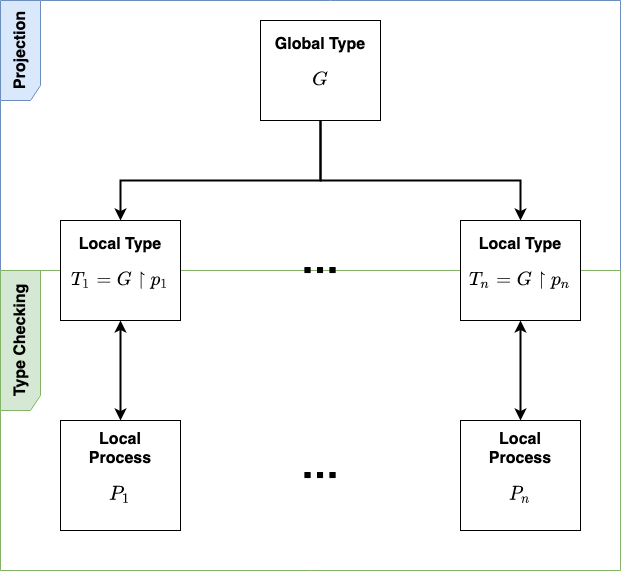
\includegraphics[width=.75\textwidth]{MpstFramework}
\caption{Type Checking with Multiparty Session Types}
\label{fig:mpstworkflow}
\end{figure}

\section{Related Work}
The two main approaches for incorporating our MPST workflow into application
development are native language support for first-class linear channel resources \cite{ATS} and code generation.
The latter closely relates to our proposal;
we highlight two areas of existing work under this approach that motivate our
design choice.

\paragraph{Endpoint API Generation}
Neykova and Yoshida targeted Python applications and the generation of runtime
monitors \cite{Python2017} to dynamically verify communication patterns.
Whilst the same approach could be applied to JavaScript, we can provide more
static guarantees with TypeScript's gradual typing system and compiler. Scribble-Java \cite{Hybrid2016} proposed to encode the EFSM
states and transitions as classes and instance methods respectively, with
behavioural typing achieved statically by the type system and channel linearity
guarantees achieved dynamically since channels are exposed and
aliasing is not monitored.
% REVIEW: could the approach of the present paper by applied to Java as well? discuss?
Scribble-Java can generate callback-style APIs similar to the approach we 
present, but this approach is arguably less idiomatic for Java developers.

\paragraph{Session Types in Web Development}
King et al. \cite{PureScript2019} targeted web development in PureScript using the
\textit{Concur UI} framework and proposed a type-level encoding of EFSMs as
multi-parameter type classes.
However, it presents a trade-off between achieving static linearity guarantees
from the type-level EFSM encoding under the expressive type system and
providing an intuitive development experience to developers, especially given
the prevalence of JavaScript and TypeScript applications in industry. Fowler \cite{MVU2019} focused on applying binary session types in front-end web
development and presented approaches that tackle the challenge of guaranteeing
linearity in the event-driven environment.

Our work applies the aforementioned approaches in a \textit{multiparty} context
using industrial tools and practices to ultimately encourage MPST-safe web
application development workflows in industry.

%\paragraph{Typestate programming} \dots



\section{TypeScript}
\label{section:typescript}

We introduce the TypeScript language 
\cite{UnderstandingTypeScript}
as our choice of target language
for session type API generation.
Developed by \textit{Microsoft Research},
TypeScript is an extension to
JavaScript to address
the deficiencies of the latter in
\textit{developing} and \textit{maintaining}
large-scale complex applications.
Syntactically,
TypeScript is a \textit{superset} of JavaScript,
so every JavaScript program is a
TypeScript program.
The TypeScript Compiler is used
to compile a TypeScript program into JavaScript
source code; since
JavaScript is a dynamically typed langauge,
the compilation process features full type erasure.

We introduce specific language
features used to implement our API generation
solution throughout the report as needed;
here, we highlight the key properties
of the type system implemented in the language.

\paragraph{Structural Typing}
In a structural type system, type equivalence
is determined by \textit{shape} rather than by name
(which is the case in a \textit{nominal} type system).

Consider the following TypeScript code:

\begin{lstlisting}[language=javascript]
class ThisSquare {
	constructor(public side: number) { }
};

class ThatSquare {
	constructor(public side: number) { }
};

declare function area(sq: ThisSquare): number;

area(new ThisSquare(2));	// ok
area(new ThatSquare(2));	// ok (*@\label{line:structural1}@*)
area({ side: 2 });			// ok (*@\label{line:structural2}@*)
\end{lstlisting}

The \texttt{area} function takes a \texttt{ThisSquare}
as parameter.
Under a structural type system,
\cref{line:structural1,line:structural2}
will type-check, because \texttt{ThatSquare} and the object
literal created from scratch matches the \textit{shape}
of \texttt{ThisSquare} -- all of them have a \texttt{side}
property typed \lstonelinejs{number}.

In languages (e.g. Java) that use a nominal type system, 
\cref{line:structural1}
will not type-check because \texttt{ThatSquare} is not named
\texttt{ThisSquare}.

\paragraph{Gradual Typing}
In a gradual type system, a program can have parts
that are statically typed and other parts are dynamically
typed \cite{GradualTyping}.
TypeScript distinguishes dynamically typed code using
the \lstonelinejs{any} type.

\begin{lstlisting}[language=javascript]
// Invoke remote API
fetch('https://jsonplaceholder.typicode.com/todos/1')
	// Convert to JavaScript Object Notation
	.then((response: Response) => response.json())
	.then((json: any) => {
		// Up to the developer to correctly deserialise;
		// incorrect implementations will cause
		// runtime type error.
	});
\end{lstlisting}

The rationale for this decision in \cite{UnderstandingTypeScript}
is that, JavaScript programs tend to interact with
data of unspecified types (such as fetching data
from API calls over the network); these parts
need to be dynamically typed in order to give developers
a smooth transition into TypeScript, and for TypeScript
to be usable in a distributed system setting. \\

\noindent
Based on the compatibility of TypeScript
with JavaScript, 
we believe that TypeScript API generation for session-typed
web development best achieves our objective
of providing
developers with a workflow
that provides communication safety guarantees in \textit{modern
web programming}
through multiparty session types.
We argue that the type system of TypeScript,
along with other language features we introduce
throughout the course of the report, is sufficient
for implementing session type theory in a manner that
complements idiomatic web development practices.



\chapter{Project Plan}
We aim to develop a multiparty session type-safe development workflow for building interactive full-stack TypeScript applications that conform to a communication protocol. This involves encoding session types using the TypeScript language and implementing a code generation workflow to generate the encodings.

\section{Delivery}
At the point of writing, we have analysed the existing code generation approaches presented in \cite{Hybrid2016, Scribble, Python2017} and assessed their applicability with respect to verifying the communication aspects of interactive web applications. We have also explored approaches for encoding session types into TypeScript, motivated by existing works along with similar proposals specific to web development in \cite{PureScript2019, MVU2019}.

We plan to deliver our code generation implementation incrementally, aiming to get a working version of the end-to-end workflow first, then iteratively add support for more complex session type primitives. This minimises the risks involved in the project by ensuring we have a functional deliverable at the early stages of the project. We plan to deliver this basic end-to-end workflow by the end of February.

The subsequent months will involve adding support for other primitives (i.e. selection, choice and recursion) for multiparty sessions. We plan to measure our progress by writing example protocols for these milestones and checking that our implementation supports those protocols by the end of each month.

We will also try to connect with web developers in the community to experiment with our implementation to get feedback on ways to make it more applicable and compatible with industry practices, such that we can apply their feedback on the next iterations of our deliverables.

If time permits, we may explore possible extensions of applying supporting \textit{Explicit Connection Actions} presented in \cite{FASE2017} in our workflow to support more protocols.

\section{Timetable}
We attach a preliminary timetable (Table \ref{table:timetable}) for guidance.

\begin{figure}
\centering
\begin{tabular}{l|p{0.4\textwidth}|p{0.4\textwidth}}
Month & Milestones & Deadlines \\
\hline\hline
Jan & \begin{itemize}
\item Explore approaches for TypeScript encoding
\item Investigate methods for code generation from EFSM
\end{itemize} & \begin{itemize}
\item 24th: Interim Report
\end{itemize} \\
\hline
Feb & \begin{itemize}
\item Develop API generation end-to-end toolchain
\item Support binary sessions with simple send/receive
\end{itemize} & \begin{itemize}
\item 2nd: PLACES 2020
\item 14th: Project Review
\end{itemize} \\
\hline
Mar & \begin{itemize}
\item Support multiparty sessions with simple send/receive
\end{itemize} & \begin{itemize}
\item 16th-20th: Examinations
\end{itemize}\\
\hline
Apr & \begin{itemize}
\item Support binary sessions with selection, choice and recursion
\item Example: calculator service
\end{itemize} & \begin{itemize}
\item 6th-17th: Easter break
\end{itemize}\\
\hline
May & \begin{itemize}
\item Support multiparty sessions with selection, choice and recursion
\item Example: Tic Tac Toe game
\end{itemize} & \begin{itemize}
\item 15th: Health check-up
\end{itemize}\\
\hline
Jun & \begin{itemize}
\item Complete report write-up
\end{itemize} & \begin{itemize}
\item 15th: Final Report
\item 26th: Final Archive
\end{itemize}
\end{tabular}
\captionof{table}{Project Timetable.}
\label{table:timetable}
\end{figure}



\chapter{Evaluation Plan}

\section{Correctness}
% Qualitatively argue how the approach achieves behavioural typing and preserves channel linearity
We will qualitatively argue how our TypeScript encodings of session types achieve behavioural typing and preserves channel linearity.

% May explore formalisms if time permits
If time permits, we may explore possible formalisms of our implementation as a calculus upon which to prove correctness. This may be related to the formal language presented in \cite{UnderstandingTypeScript}, but we will need to extend this to be specific to our TypeScript encodings of session types.

\section{Productivity} 
% Compare with PureScript implementation to talk about developer productivity when using PureScript APIs with ConcurUI compared to TypeScript APIs when using React
By adopting tools and practices used in industry, we wish to assess the extent to which our implementation boosts developer productivity by providing APIs that guarantee communication protocol conformance in a way that is compatible with existing workflows. Comparing the development workflow of implementing the \textit{Battleships} game using the PureScript workflow in \cite{PureScript2019} and our TypeScript-based proposal would yield interesting findings.

% Survey - qualitative and quantitative feedback
This can be carried out as a survey to be completed by web developers familiar with both languages. We would include questions that allow us to collect both qualitative and quantitative feedback to make effective comparisons between our approach and existing proposals.

\section{Performance} Examples of performance metrics include: lines of code to be written by the developer (as a result of using the generated APIs), the size of the transpiled JavaScript assets to be loaded on the server and client browsers. We aim to extract these metrics from our approach and compare them against metrics extracted from a baseline implementation (i.e. without using the MPST methodology) and evaluate the performance overhead (if any) of our MPST-based approach.

\clearpage

\bibliographystyle{acm}
\bibliography{report}

\end{document}
%%% Local Variables: 
%%% mode: latex
%%% TeX-master: t
%%% End: 
